\documentclass[12pt, a4paper]{pancake-article}

\usepackage{mathtools}

\usepackage{fontspec}
\usepackage{unicode-math}
\setmathfont{TeX Gyre Termes Math}
\setmainfont{TeX Gyre Termes}[Ligatures=TeX]
\setsansfont{TeX Gyre Heros}[Ligatures=TeX]
\setmonofont{DejaVu Sans Mono}[Ligatures=TeX]

\usepackage{graphicx}

\usepackage[
	style=apa
]{biblatex}
\addbibresource{Bibliography.bib}

\usepackage{setspace}
\doublespacing

\usepackage{siunitx}
\sisetup{mode=math}

% colors!
\usepackage[usenames, dvipsnames]{xcolor}
\newcommand{\tint}[1]{{\color{accent}#1}}

\usepackage{hyperref}
\hypersetup{
	hidelinks,
	colorlinks,
	breaklinks=true,
	urlcolor=accent,
	citecolor=accent,
	linkcolor=accent,
	bookmarksopen=false,
	pdftitle={Sorting sentiments of hotel reviews through machine learning},
	pdfauthor={Darren Yap},
}

\title{Sorting \tint{sentiments} of hotel reviews through \tint{machine learning}}
\author{\tint{Yap} Hao Ming Darren \and \tint{Tan} Jia He \and \tint{Fu} Jinghang}
\date{\scshape Singapore Mathematics Project Festival 2024}

% start the document!
\begin{document}

\maketitle
\thispagestyle{empty}
\pagebreak
\setcounter{page}{1}
\tableofcontents

% ** abstract **
\begin{abstract}
	Hotels depend on tourists to survive. They gather consumer opinions via customer
	reviews to improve their services. This project used sentiment analysis---the
	process of determining the emotional tone of text---to quantify consumers'
	opinions on hotels, and predicted the overall sentiment of hotel reviews.
	International hotel reviews in English were split into individual words,
	assigning each word a score based on its relative intensity. The sentiment
	makeup of the review dataset was highlighted and the most frequent tokens were
	identified. Two machine learning models---a logistic regression model and a random
	forest classifier---were also constructed to predict the overall sentiment of a
	review. It was shown that the models were capable of predicting the overall
	sentiment of hotel reviews. This project highlights the possibility of using
	sentiment analysis models to create applications that allow customers to better
	understand the perceived quality of a hotel and potentially combat review fraud---the
	the dishonest practice of manipulating false reviews to boost a hotel's ratings.
\end{abstract}

\section{Introduction}
After the Singapore government relaxed travel restrictions due to COVID-19,
there has been a recent increase in the number of tourists travelling in and out of Singapore.
As such, hotels have seen a rise in the number of prospective tourists to be housed,
and this may encourage an increase in the number of reviews hotels may receive.

Today, it is common to use social networks, messengers, and review websites
to receive data from customer opinions. This is especially true for hotels,
where previous occupants may evaluate the hotel on several factors through their
reviews---be it cleanliness, facilities, location and convenience, etc.
These come in two forms---a quantitative review (based on stars, diamonds,
hearts, etc.) and a more qualitative review through text.

However, quantitative reviews do not always paint the full picture of customers'
opinions towards a certain hotel. Though it is certainly helpful to have a more
objective rating system using numerical scores, eg. the Department of Tourism
grading system in the Philippines, or the European \textit{Hotelstars} Union system,
these are given by customers subjectively and do not reflect the reasons for
customers giving the rating. There is also evidence of manipulation of ratings
by hotel management itself, where hotels may be compelled to forge positive or
negative ratings to bias the overall rating. This made up \qty{2.1}{\percent}
of the 66 million reviews submitted to TripAdvisor in 2019 (\cite{tripadvisor}).
Therefore, we propose using sentiment analysis to extract customers' true
feedback on hotels instead.

\section{Research Questions and Hypotheses}
The following were investigated, in increasing order of difficulty:
\begin{enumerate}
	\item How could the sentiments of individual words be quantified on a numerical scale?
	\item How could the sentiments of paragraphs be quantified on a numerical scale?
	\item How could tokens in hotel reviews be used to predict the overall sentiment of the review?
\end{enumerate}

The objectives of this research were as such:
\begin{enumerate}
	\item To run sentiment analysis on individual words and quantify them on a numerical scale
	\item To run sentiment analysis on paragraphs and quantify them on a numerical scale
	\item To use sentiment analysis on hotel reviews to determine consumers' overall opinions of hotels
\end{enumerate}

\section{Literature Review}
Sentiment analysis is a field of study which utilises computational methods to analyse text,
and then determine the underlying emotion it contains; at simple levels, text can be classified
into positive and negative polarities; at more complex levels, more specific emotions, such as
\textit{happy}, \textit{sad} and \textit{angry}, can be determined. It
has broad applications which range from determining consumers' opinions in sales and product
analysis to competitor research in marketing, and even detecting public opinion in social media
monitoring. Sentiment analysis will be used in this research to analyse hotel occupants' reviews
and determine their sentiments towards them, without interference from human bias.

\citeauthor{stock} (\citeyear{stock}) predicted the stock market opinion of StockTwits communities of expert
investors. Sentiment analysis was used in a deep learning model to extract sentiment from Big Data.
A Pearson Correlation Coefficient combined the linear correlation between users' sentiment and
future stock prices, which showed that the accuracy of user sentiment was \qty{53}{\percent}. It was
concluded that convolutional neural networks could predict stock market movement based on
sentiment.

Using the social networking site Twitter, \citeauthor{twitter} (\citeyear{twitter}) determined
Filipinos' sentiment in response to the Philippine government's efforts at tackling COVID-19,
specifically the implementation of vaccination. Sentiment analysis was used to extract sentiment
from text in the English and Tagalog languages, the results from which were used to train a Naïve
Bayes model. A confusion matrix was produced, representing the model's prediction accuracy
in classifying sentiment into positive, neutral and negative categories---\qty{81.77}{\percent}.
It was concluded that sentiment analysis was sufficiently accurate to help the Philippine government
better conduct budget planning and coordinate COVID-19 efforts.

\citeauthor{spain} (\citeyear{spain}) analysed tourism quality in Spain
by extracting sentiment from reviews by Chinese tourists on the tourism
social networking sites Baidu Travel, Ctrip, Mafengwo, and Qunar.
Two sentiment analysis methods, lexicon-matching and corpus-based machine
learning methods, were used. These methods allow for the processing of
unstructured text of comparatively longer lengths. Clustered data
visualisation categorised aspects of Spanish tourism into positive
and negative groups, with the majority residing within positive sentiment.
It was concluded that sentiment analysis can be used to improve tourism
quality and sustainability decision-making.

SentiStrength, a tool for lexical sentiment analysis---sentiment analysis
done on short, low quality texts---was used to study emotions expressed
in GitHub commit comments of different open-source projects (\cite{github}).
Each word was assigned a score, then the net score for each comment was calculated.
Eacch comment was split into snippets using SentiStrength, then assigned a score by
computing the maximum and minimum scores of the sentences it contains.
Following which, the average of the positive and negative scores was taken as the
sentiment score of the entire commit. This study showed that Java projects warranted
more negative comments, and projects which had more distributed teams tended
to warrant higher positive sentiments.

In conclusion, the literature reviewed showed many possible applications
of sentiment analysis in quantifying the underlying emotion of feedback
on online platforms. Lexicon-based sentiment analysis, which assigns each
word a sentiment, then calculates a sentence's total sentiment score, can
be used, due to its simplicity in implementation, and the availability of
many open-source sentiment lexicons. In addition, sentiment categorisation
using lexicon-based sentiment analysis makes accurate predictions upwards of
\qty{70}{\percent} of the time (\cite{khoo}). SentiStrength would also be useful for
detecting sentiment from hotel reviews which are usually short in length quickly
and efficiently, facilitating the process of extracting sentiment from tourists'
reviews of hotels. Using SentiStrength for sentiment calculation is also
rather accurate, generating both positive and negative sentiments with a more
than \qty{60}{\percent} accuracy (\cite{thelwall}). Therefore, the strategies listed
above could be adopted or emulated on a smaller scale for this project.

\section{Methods and Results}

\subsection{Token-based sentiment analysis}\label{sec:tokens}
After collecting an open-source dataset of international hotel reviews in English from Datafiniti,
the reviews were tokenised and split into individual tokens. The Afinn lexicon was then obtained,
which was used to assign each token a single integer score, ranging from \(\left[-5, -1\right]\) for
negative tokens, and \(\left[1, 5\right]\) for positive ones. It was found that the vast majority
of tokens in the dataset held a positive sentiment  after a large number of neutral tokens were disregarded
(Figure~\ref{fig:bars}). The high number of neutral tokens can be attributed to nouns
describing the hotel, like \textit{food}, \textit{hotel} and \textit{pool}.

\begin{figure}[htpb]
	\centering
	\begin{minipage}{0.5\textwidth}
		\centering
		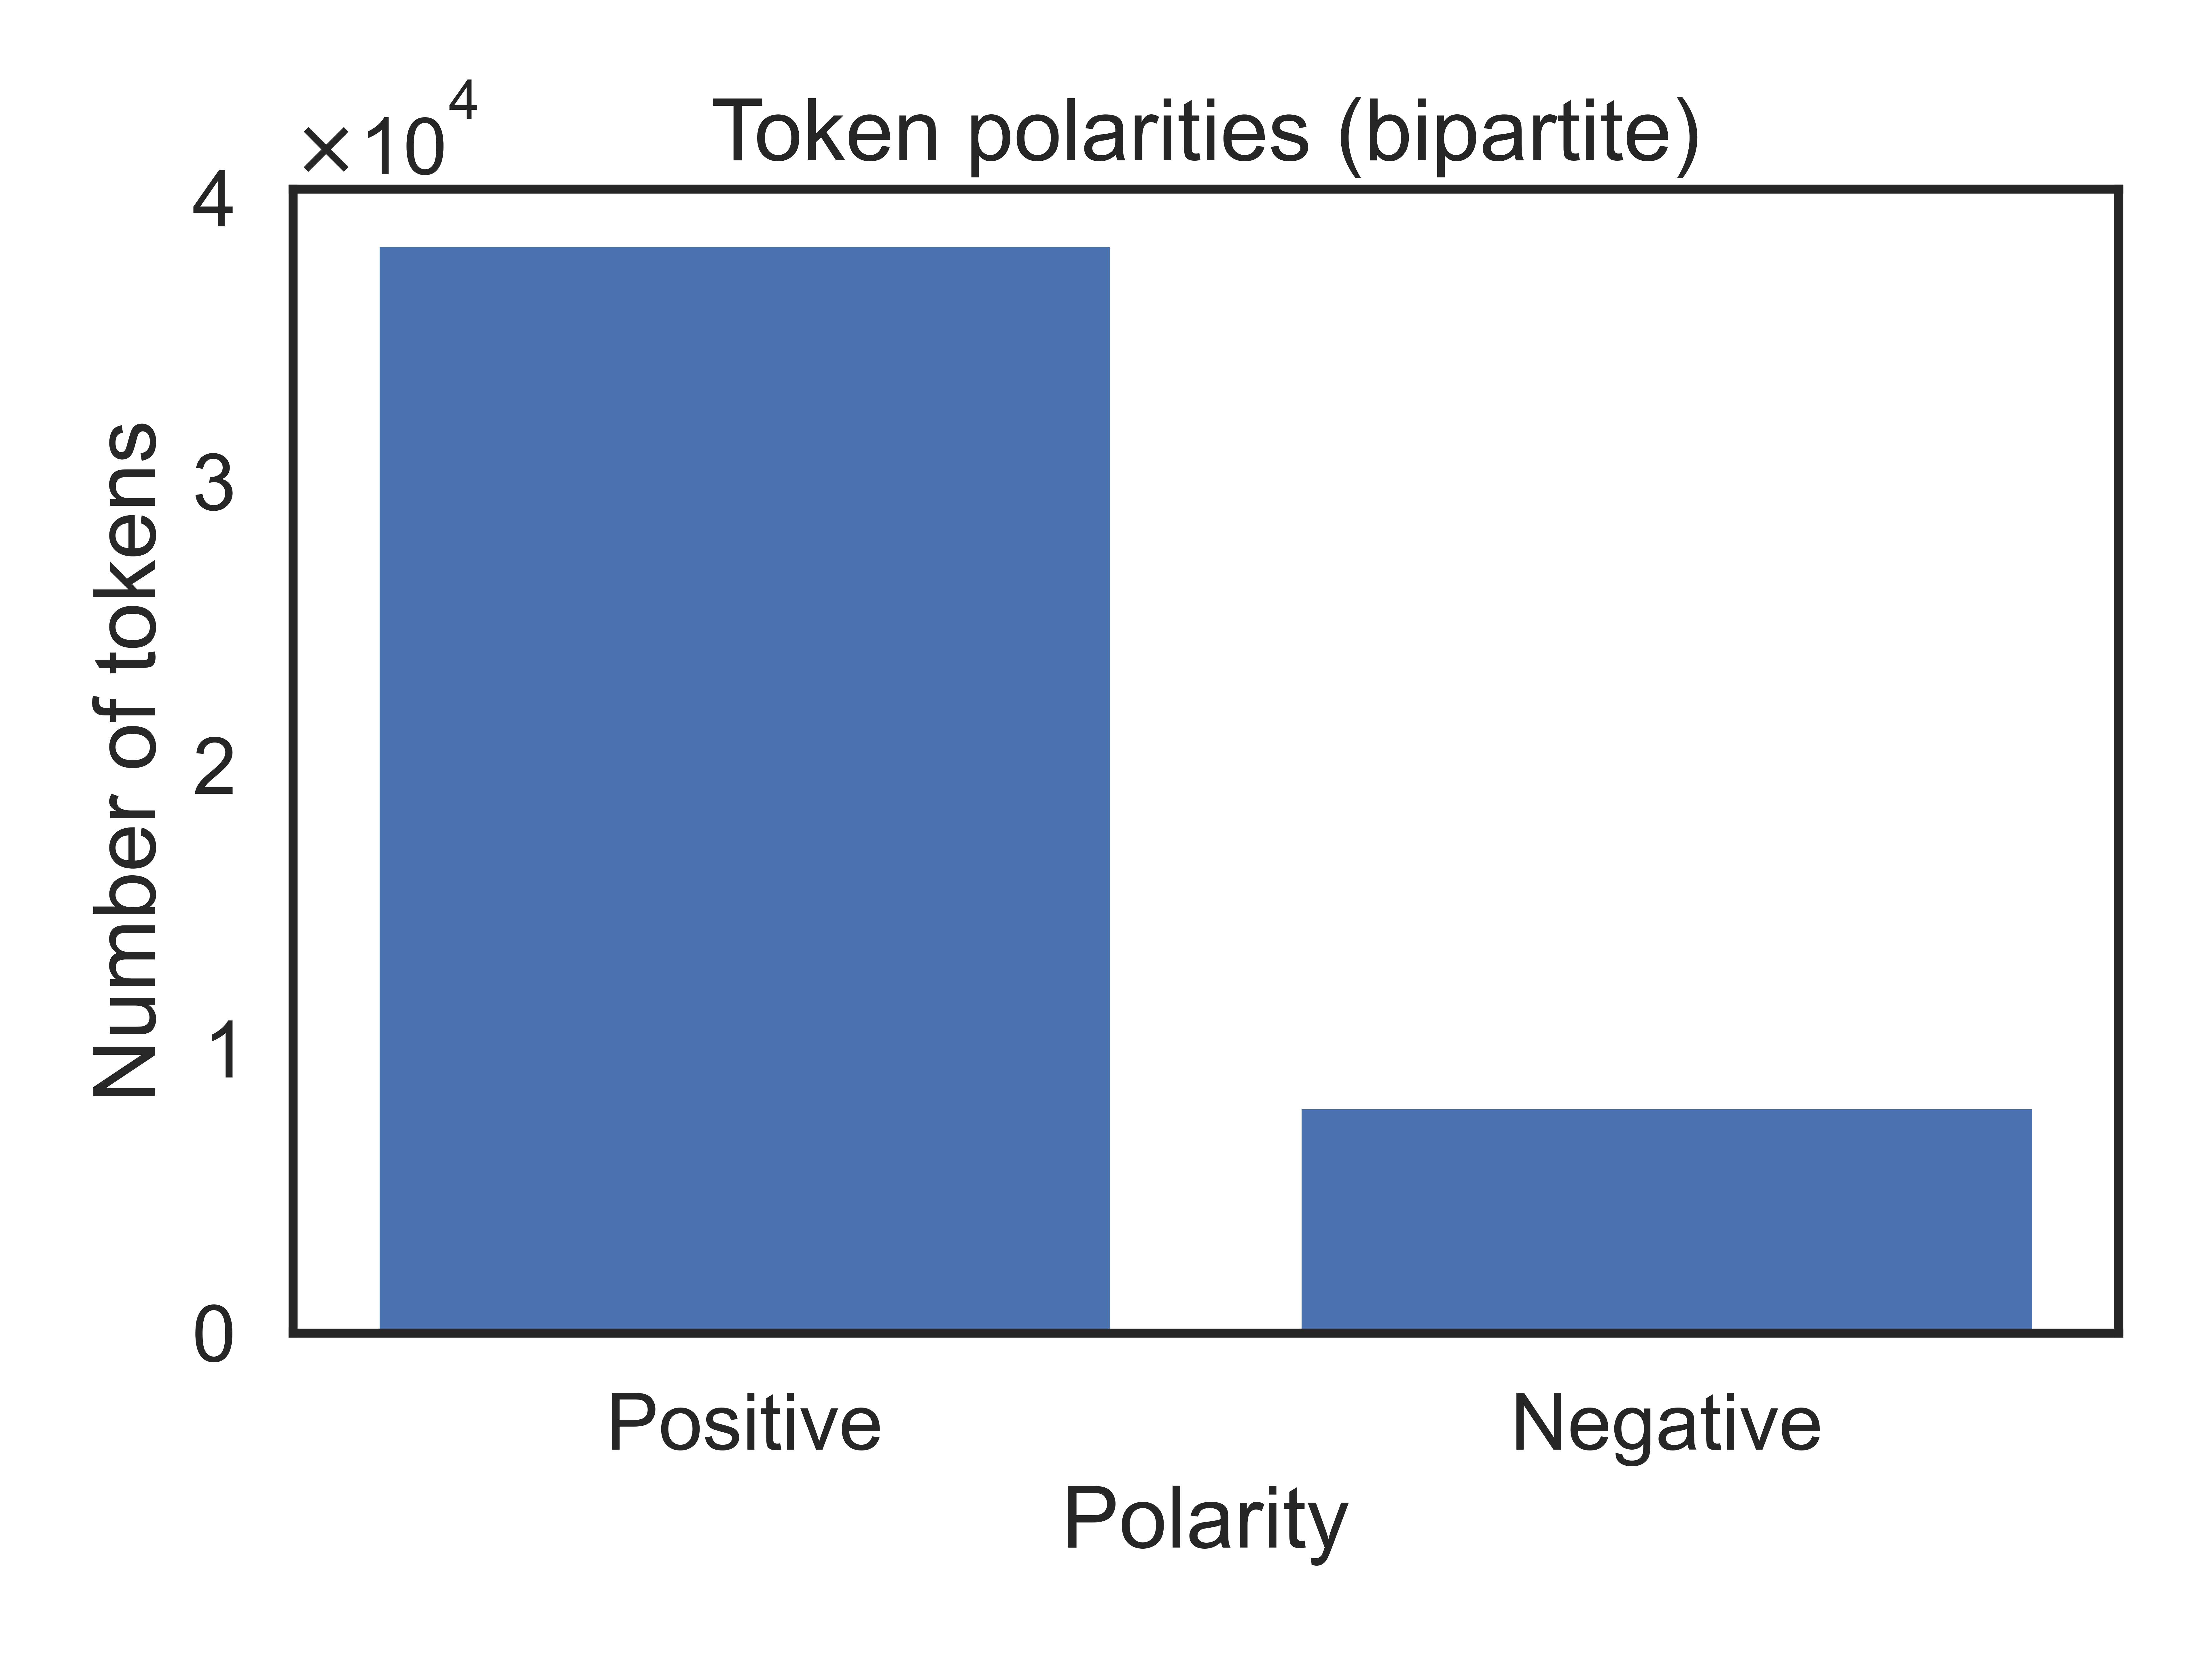
\includegraphics[width=\textwidth]{./gfx/rq1/bar_bipartite.png}
		\caption*{Bipartite sentiment}
	\end{minipage}\hfill
	\begin{minipage}{0.5\textwidth}
		\centering
		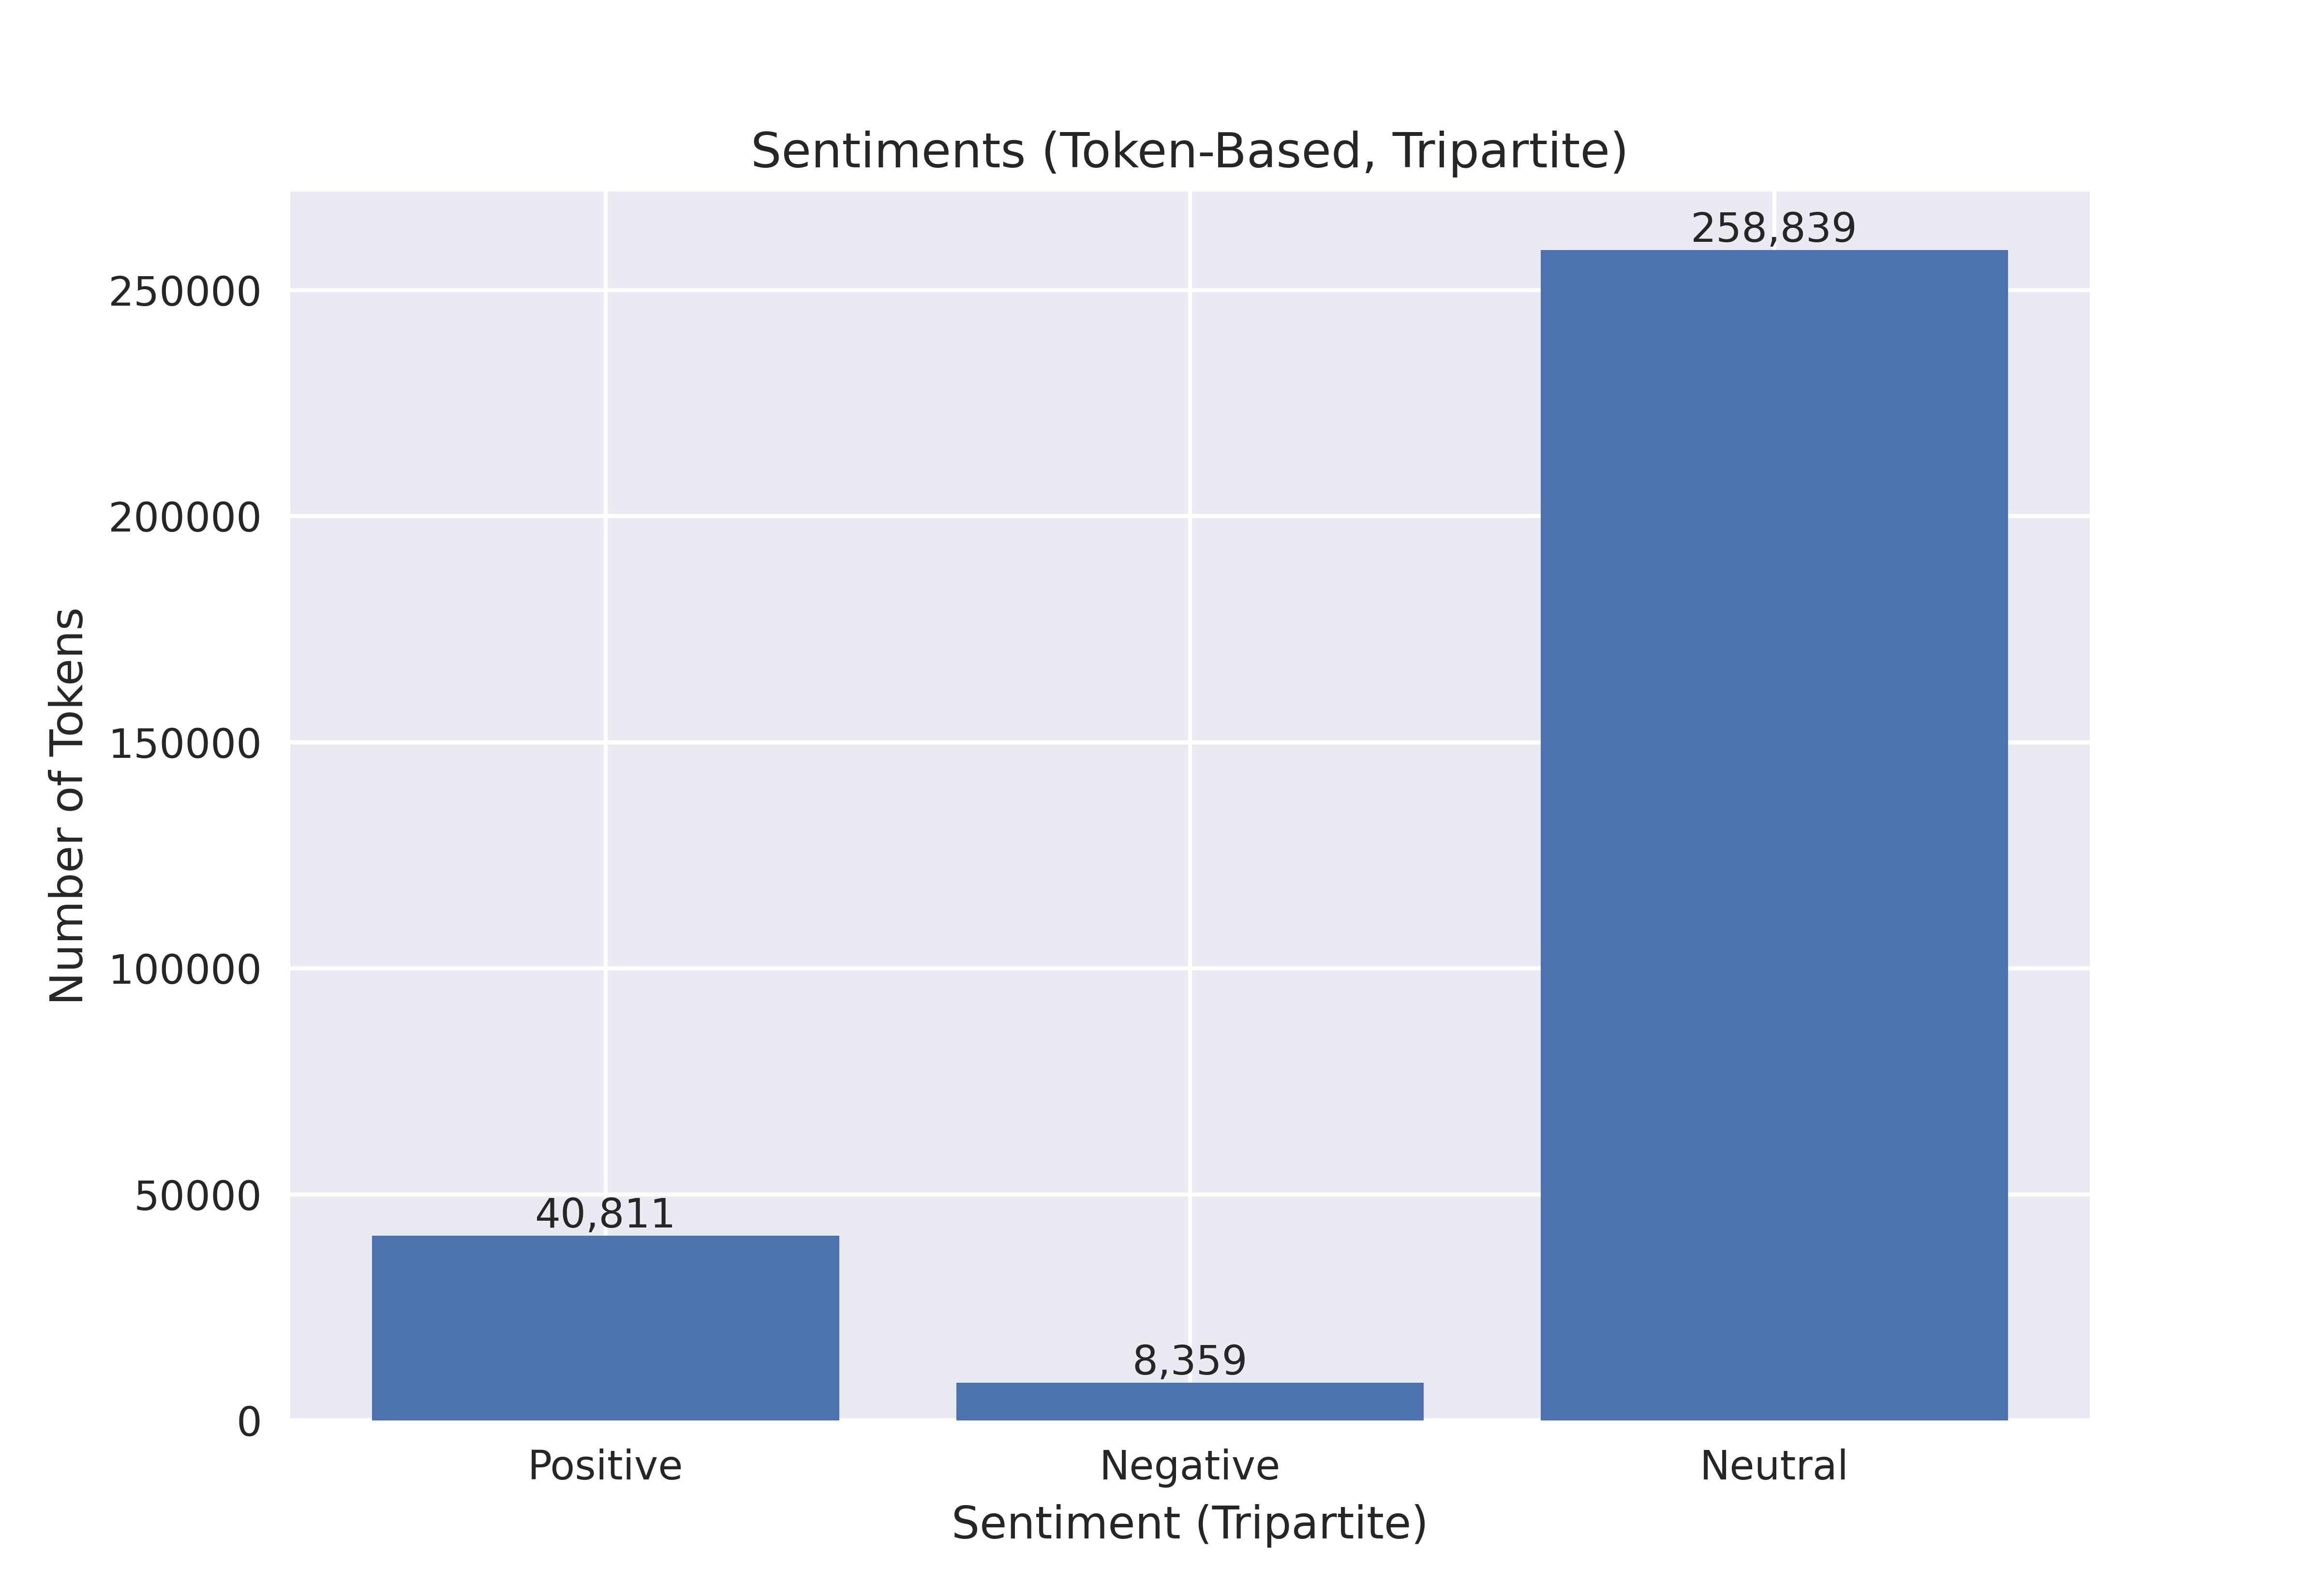
\includegraphics[width=\textwidth]{./gfx/rq1/bar_tripartite.png}
		\caption*{Tripartite sentiment}
	\end{minipage}
	\caption{Proportion of tokens by polarity}
	\label{fig:bars}
\end{figure}

It is also noted that generic tokens associated with ``goodness'' are more
prominent when discussing a hotel's desirable traits, such as \textit{great},
\textit{good} and \textit{nice}, whereas visitors were more likely to
describe the hotel in detail when criticising it, citing traits like
\textit{dirty}, \textit{noisy} and \textit{hard} (Figure~\ref{fig:wordclouds}).

\begin{figure}[htpb]
	\centering
	\begin{minipage}{0.5\textwidth}
		\centering
		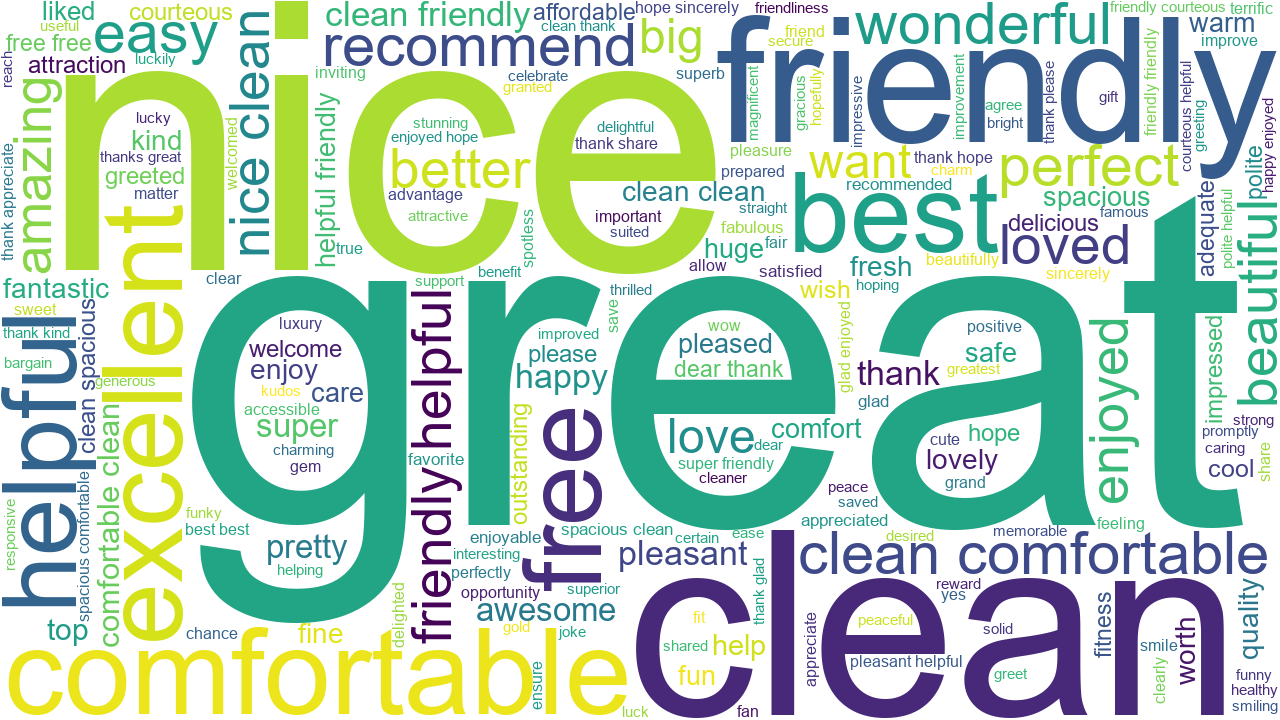
\includegraphics[width=0.9\textwidth]{./gfx/rq1/wordcloud_1.png}
		\caption*{Positive tokens}
	\end{minipage}\hfill
	\begin{minipage}{0.5\textwidth}
		\centering
		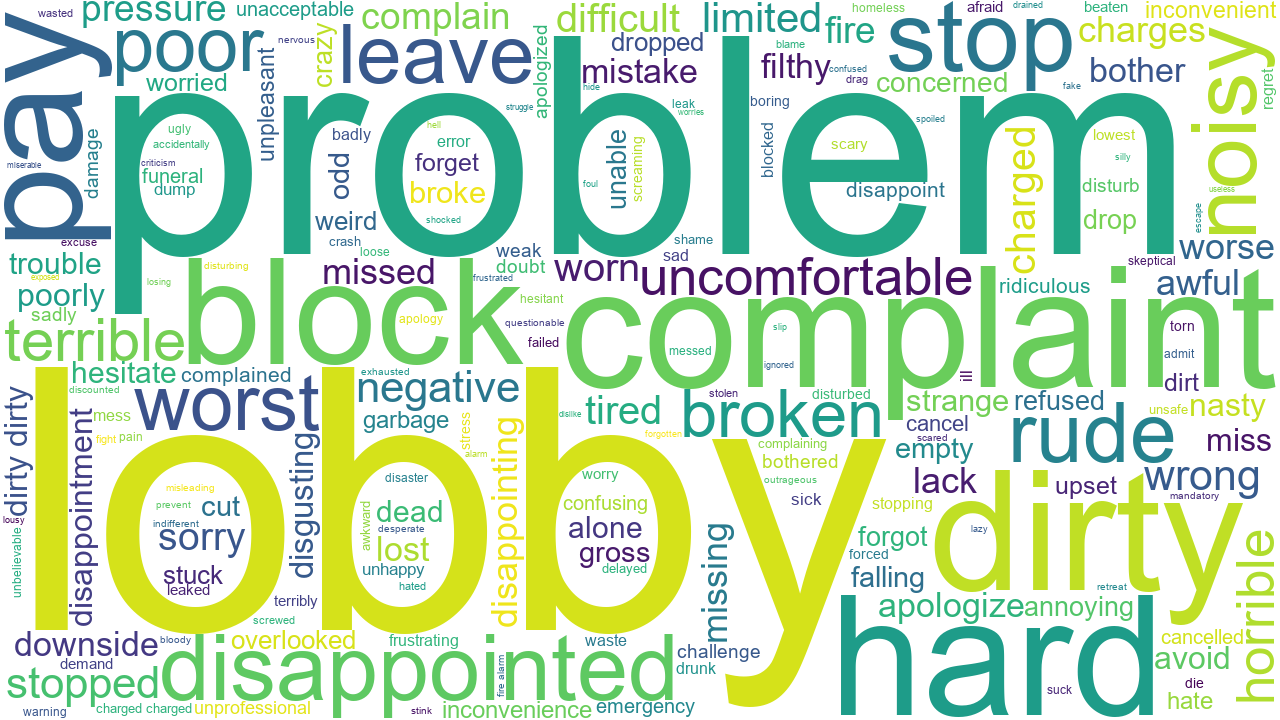
\includegraphics[width=0.9\textwidth]{./gfx/rq1/wordcloud_0.png}
		\caption*{Negative tokens}
	\end{minipage}
	\caption{Wordclouds of tokens by polarity}
	\label{fig:wordclouds}
\end{figure}

\subsection{Review-based sentiment analysis}\label{sec:reviews}

The software SentiStrength was used to generate two scores for each review:
a positive one in the range \(\left[1, 5\right]\) and a negative one in the range \(\left[–5, –1\right]\).
The greater the tonal intensity of a word, the greater the magnitude of the sentiment score
it would contribute to the overall positive or negative score of the review. Punctuation marks for
emphasis were also considered. After this, the reviews were classified into two categories: overall
positive (polarity \(1\)), and negative (polarity \(0\)). Where \(y\) is the polarity
of a review, and \(s_+\) and \(s_-\) are the positive and negative sentiment scores (Equation~\ref{eq:polarity}):

\begin{equation}
	y = \begin{cases}
		1 & s_+ + s_- \geq 0 \\
		0 & s_+ + s_- < 0    \\
	\end{cases}
	\label{eq:polarity}
\end{equation}

It is observed that a large proportion of reviews were overall positive (\qty{70}{\percent})
and only a handful of negative reviews were present (\qty{13}{\percent}) in the dataset.
Though neutral reviews may seem to make up a sizeable proportion of the reviews, this merely
shows that the magnitude of the positive and negative sentiment scores is equal (Figure~\ref{fig:pies}).

\begin{figure}[htpb]
	\centering
	\begin{minipage}{0.5\textwidth}
		\centering
		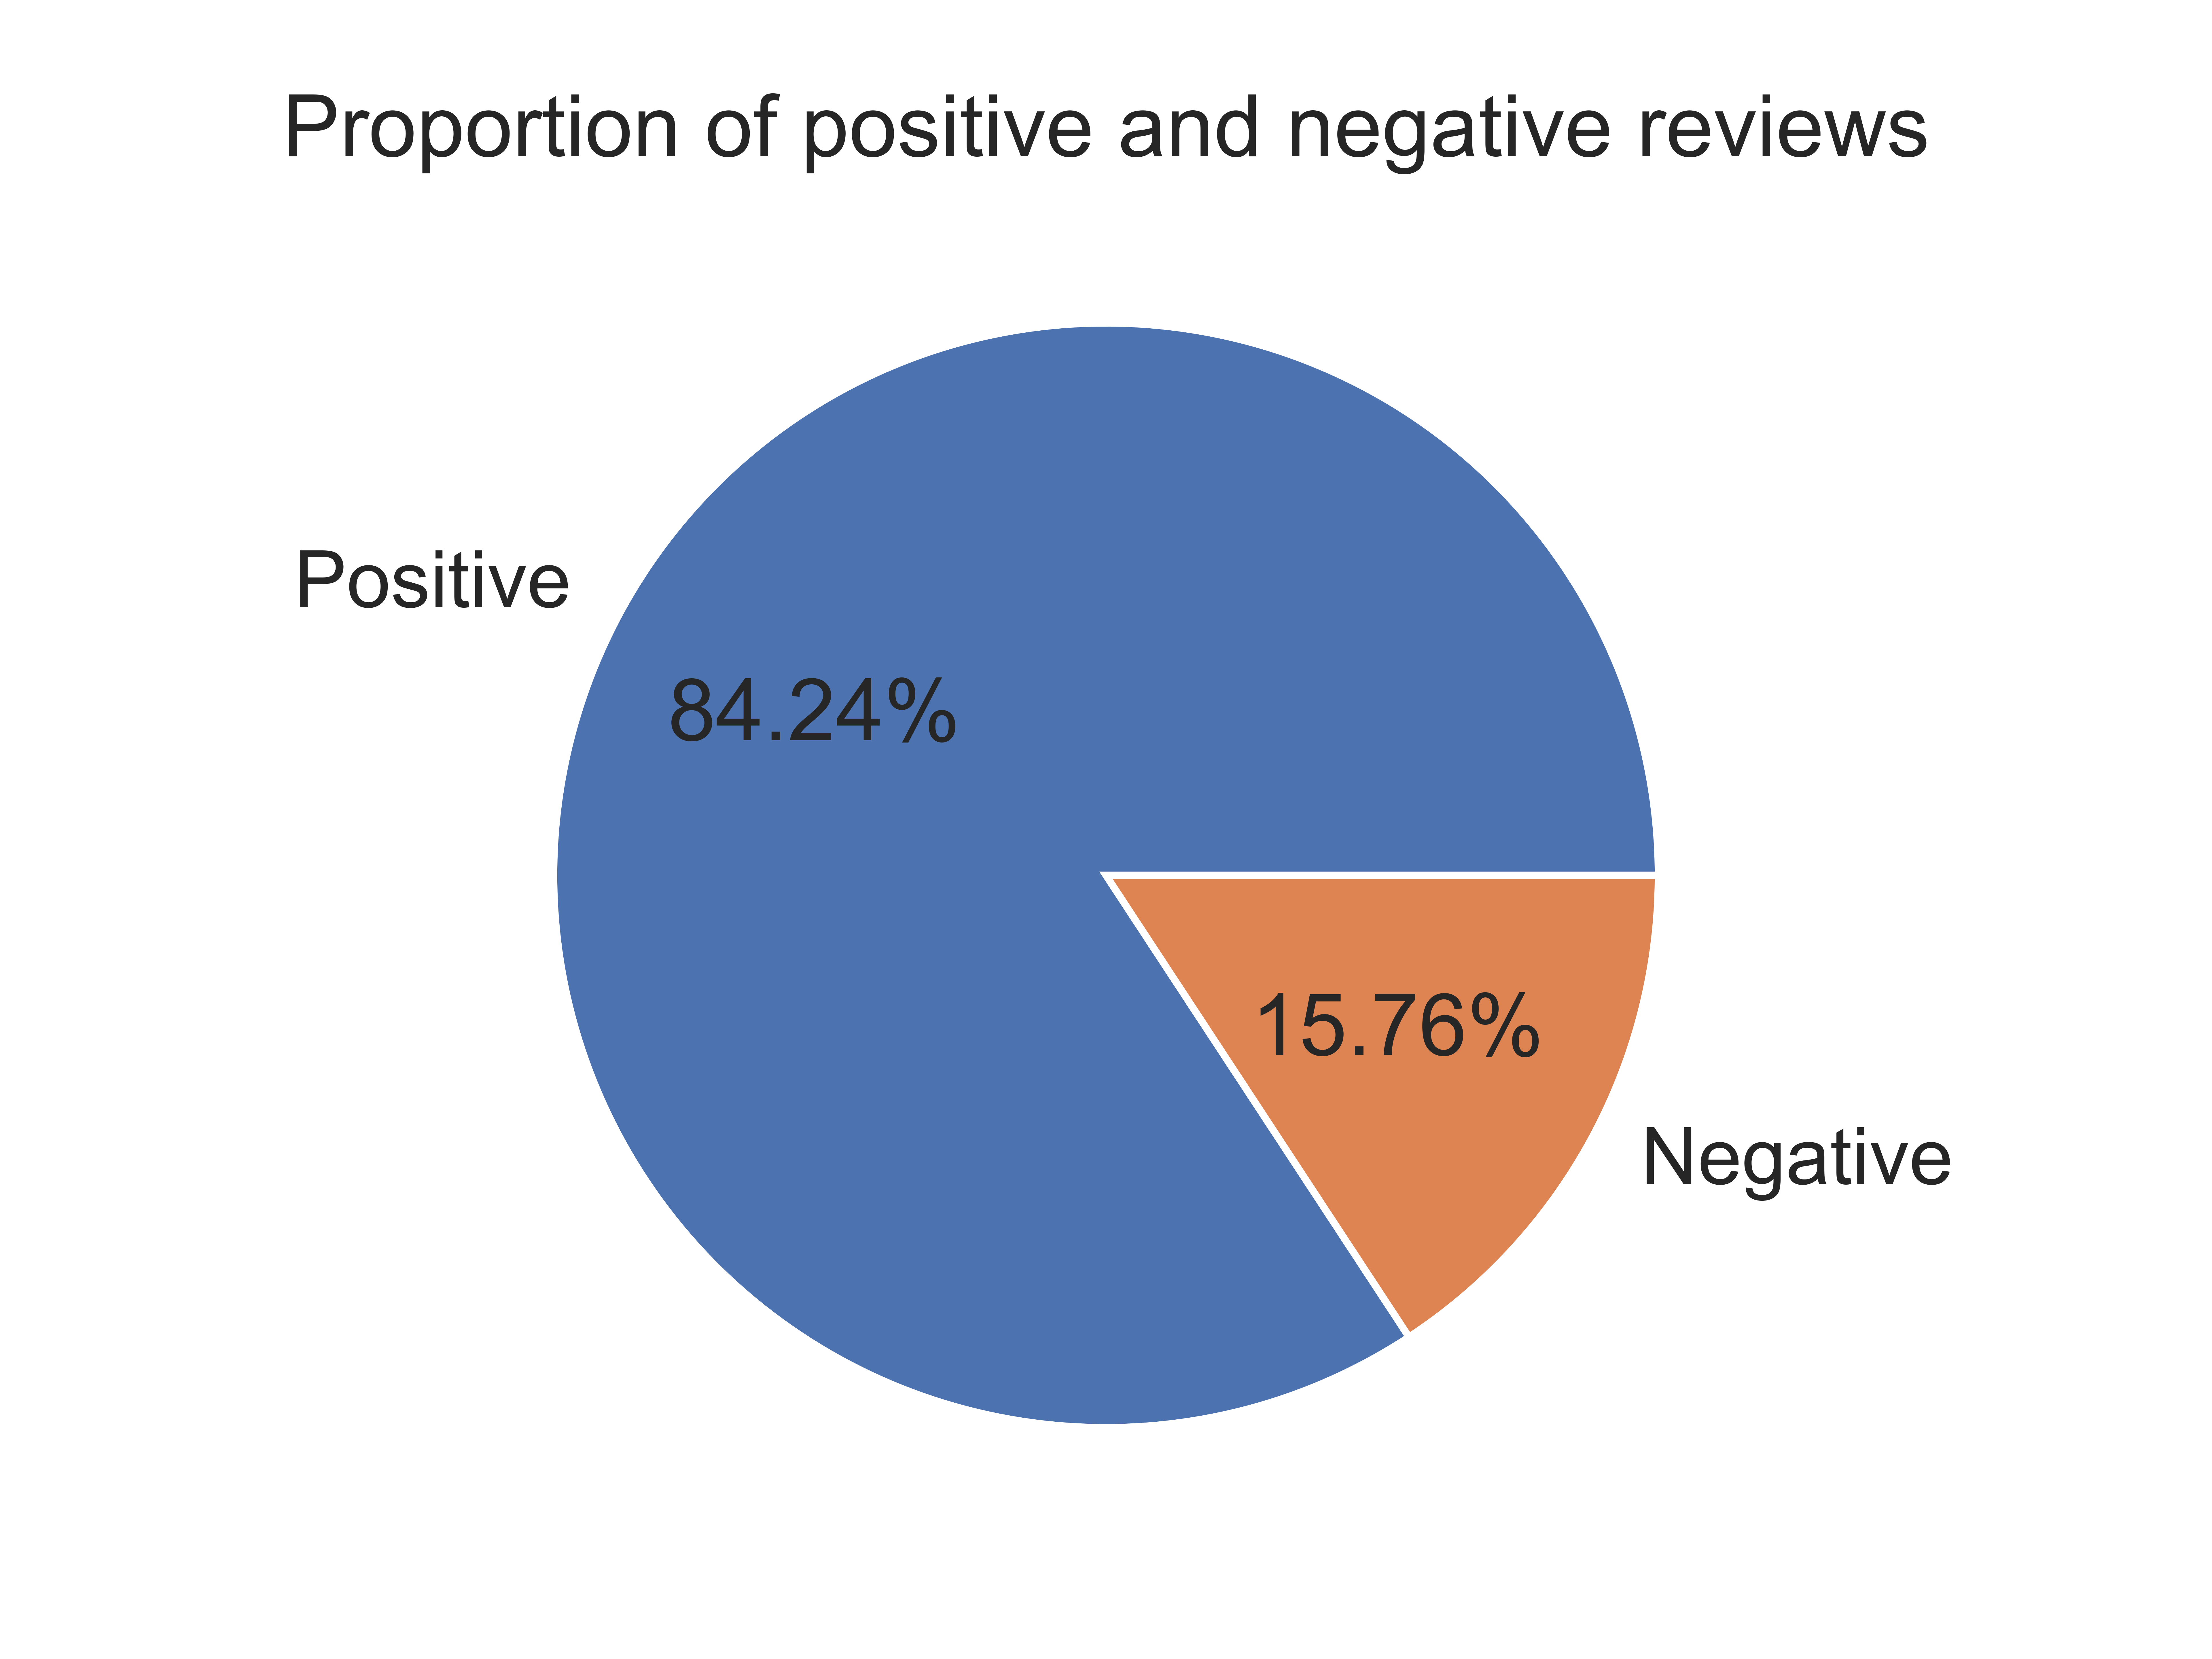
\includegraphics[width=0.9\textwidth]{./gfx/rq2/pie_bipartite.png}
		\caption*{Bipartite sentiment}
	\end{minipage}\hfill
	\begin{minipage}{0.5\textwidth}
		\centering
		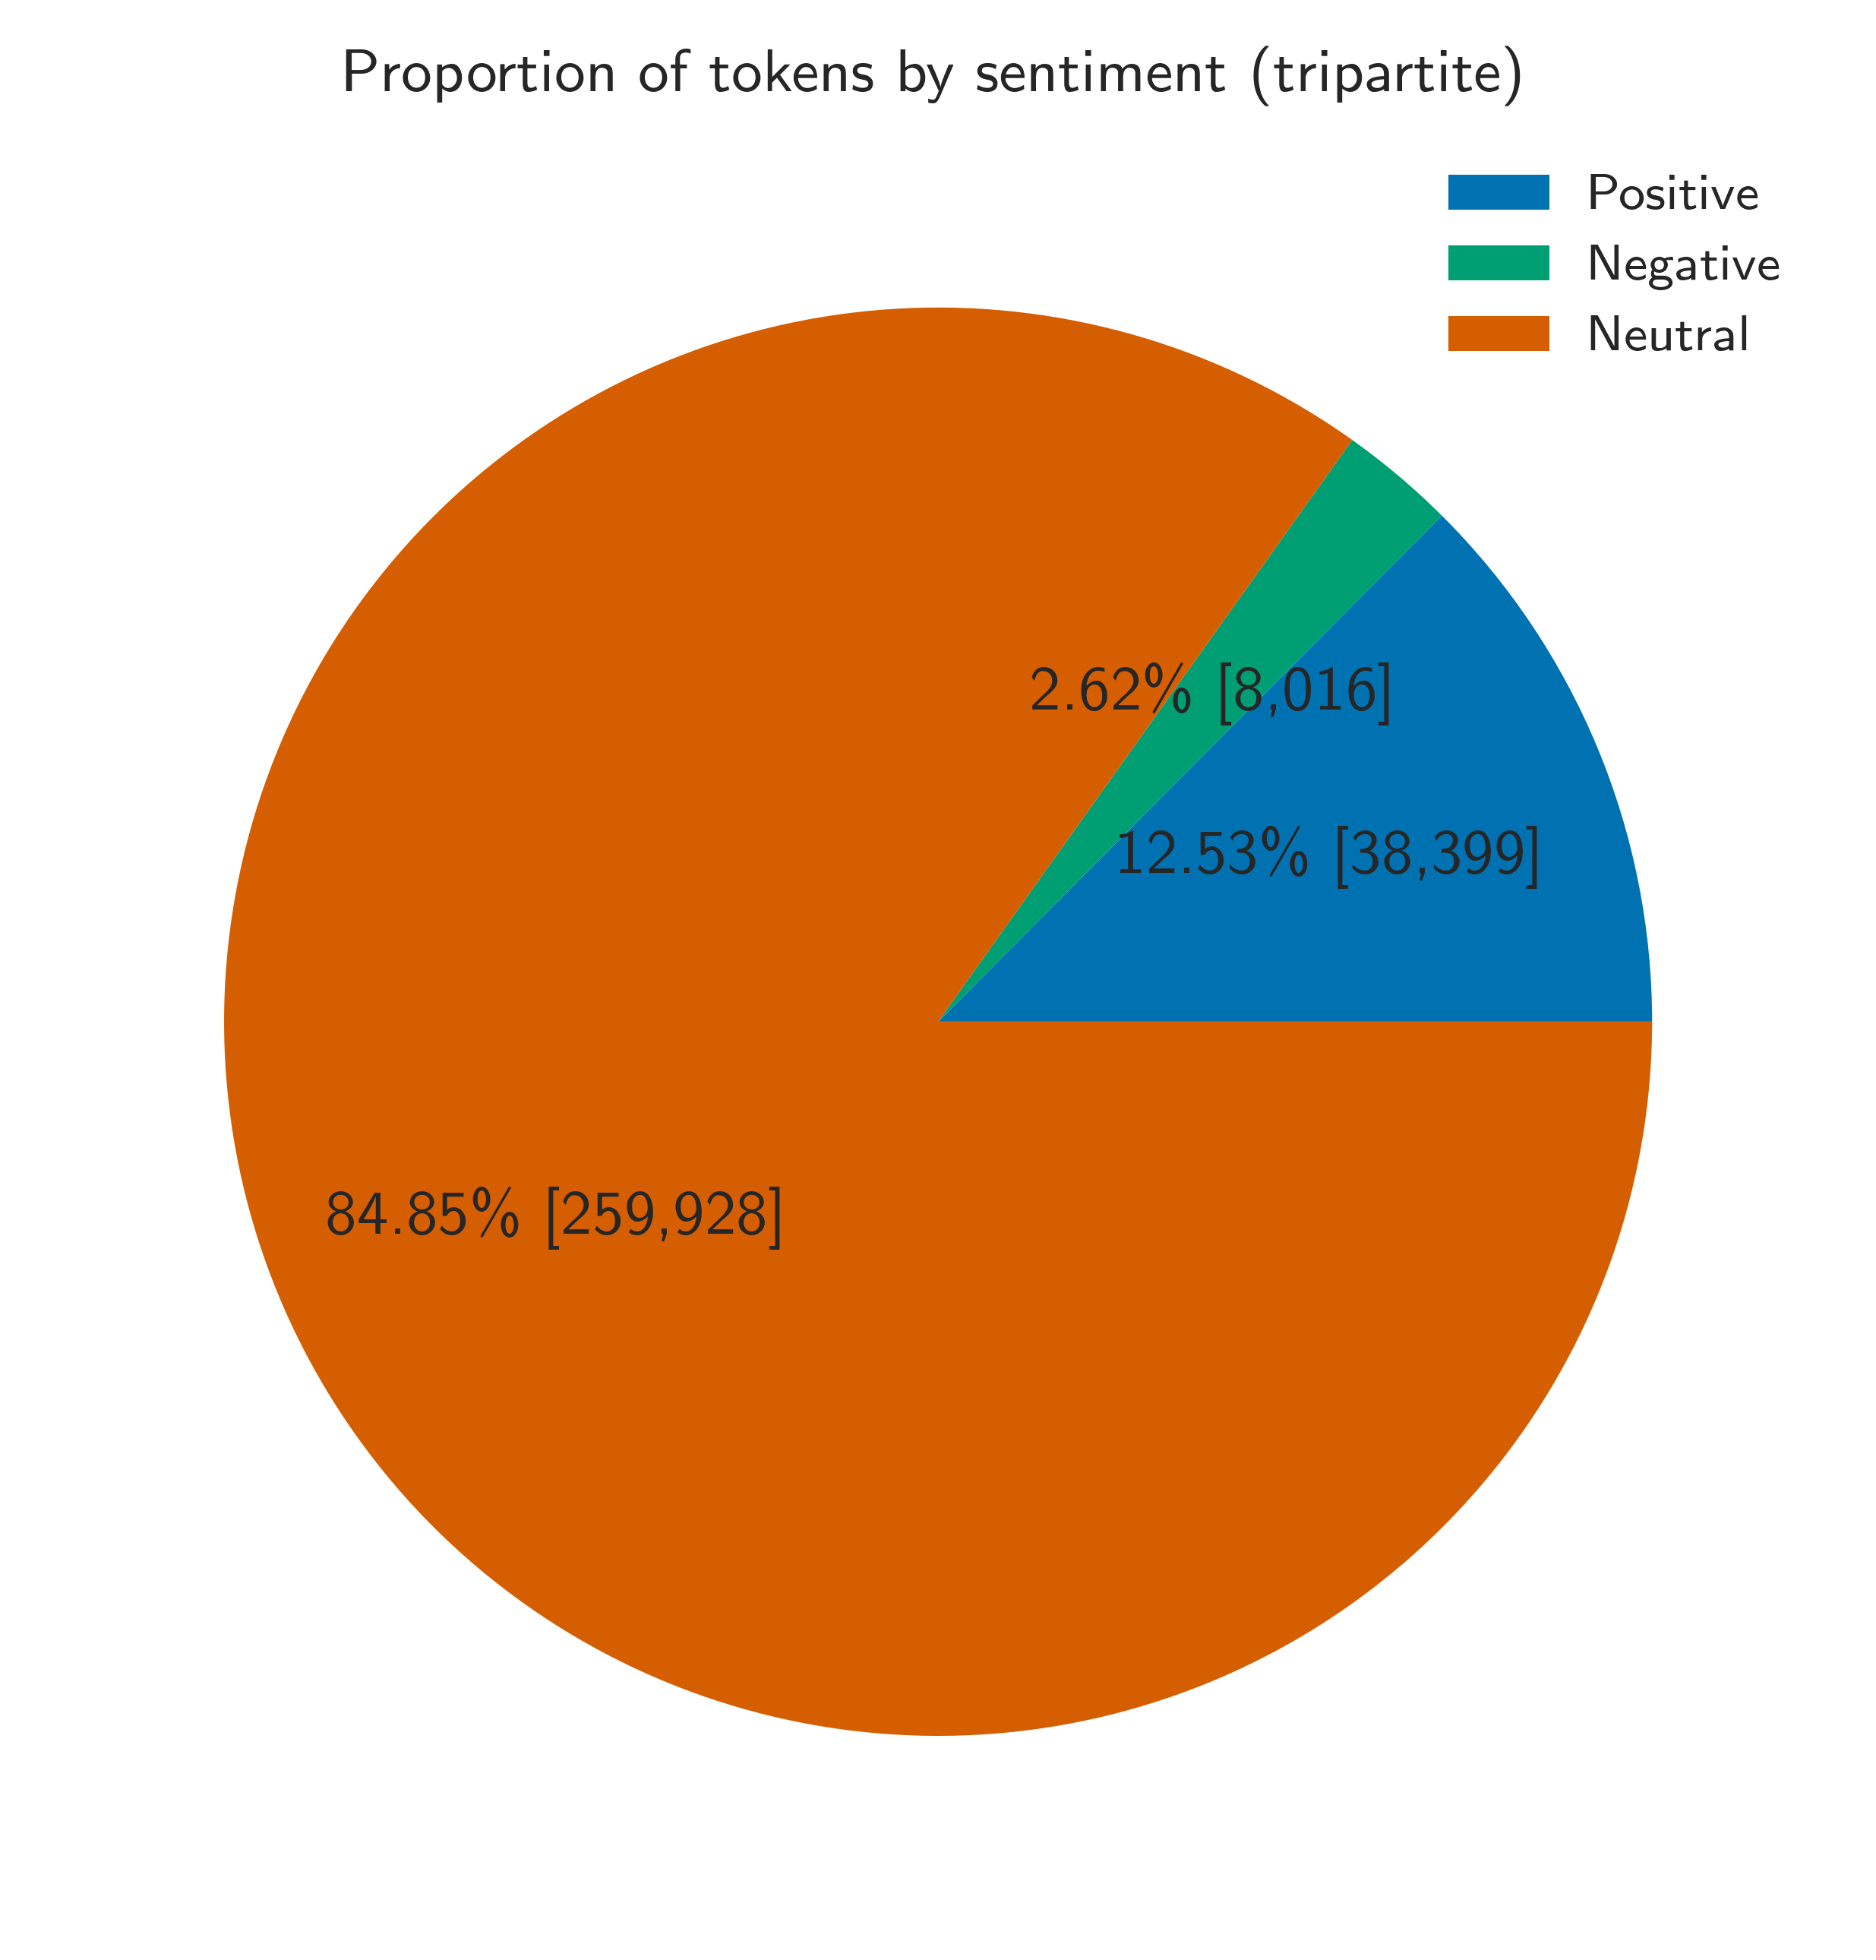
\includegraphics[width=0.9\textwidth]{./gfx/rq2/pie_tripartite.png}
		\caption*{Tripartite sentiment}
	\end{minipage}
	\caption{Proportion of reviews in dataset by polarity}
	\label{fig:pies}
\end{figure}

\subsection{Predicting sentiment via token frequency}

A frequency table for all reviews was generated, showing how
often a review (with a overall score, \(s_+ + s_-\), between \(\left[-5, 5\right]\))
occurred in the dataset. Reviews of overall neutral score were also considered.
The results here are consistent with those earlier (Section~\ref{sec:reviews}),
where positive reviews of a moderate overall score made up the majority (Figure~\ref{fig:distribution}).

\begin{figure}[htpb]
	\centering
	\includegraphics[width=0.95\textwidth]{./gfx/rq3/distribution.png}
	\caption{Distribution of reviews by sentiment score}
	\label{fig:distribution}
\end{figure}

For each review, a feature vector was constructed, which shows how
often each token in a review occurs within that review---the term frequency
of the token (Equation~\ref{eq:term-frequency}). \(\text{tf}\left(t, d\right)\)
represents the relative term frequency of token \(t\) in review (or \textit{document})
\(d\). \(f_{t, d}\) is the raw count of a token in a review.

\begin{equation}
	\text{tf}\left(t, d\right) = \frac{f_{t, d}}{\sum_{t' \in d}^{}f_{t',d}}
	\label{eq:term-frequency}
\end{equation}

It is noted that the denominator is simply the total number of token in document \(d\),
counting each occurrence of the same token separately.

To evaluate the relevance of a token \(t\) in determining the overall sentiment of the
review \(d\) in a corpus of reviews \(D\) of size \(N\), the term frequency-inverse document frequency
(tf--idf value) is found (Equation~\ref{eq:tf-idf}), where

\begin{equation}
	\text{tfidf}\left(t, d, D\right) = \text{tf}\left(t, d\right)\log\frac{N}{1 + \left|\left\{d \in D : t\in d\right\}\right|}
	\label{eq:tf-idf}
\end{equation}

\(\left|\left\{d \in D : t \in d\right\}\right|\) is the number of reviews in which token \(t\) occurs.
Since the denominator will be \(0\) if the token does not appear in the review at all, \(1\) is added
to avoid a division-by-zero.

\subsubsection{Logistic regression}

A logistic regression model was constructed to predict whether a review carries a positive or negative sentiment,
with tf--idf values ($x$) being the independent variable and the polarity of a review ($y$) being the
dependent variable.
A conventional sigmoid function was used to evaluate the probability of a review being positive, in the range
\(\left[0, 1\right]\) (Equation~\ref{eq:sigmoid}), where \(x_i\) is the tf--idf value of token \(t_i\) in
review \(d_i\):

\begin{equation}
	h\left(x_i\right)	= \frac{1}{1 + e^{-\left(\beta_0 + \beta_1 x_i\right)}}
	\label{eq:sigmoid}
\end{equation}

Here, \(\beta_0 + \beta_1 x_i\) is an arbitrary linear function of tf--idf \(x_i\), chosen
such that the loss, \(l_i\), is minimised. Let \(y_i\) be the actual polarity of review \(i\),
determined through Equation~\ref{eq:polarity}.

The loss, \(l_i\), for the \(i\)-th tf--idf value is given as (Equation~\ref{eq:logloss}):
\begin{equation}
	l_i = \begin{cases}
		- \ln h_i                  & y_i = 1 \\
		- \ln \left(1 - h_i\right) & y_i = 0 \\
	\end{cases}
	\label{eq:logloss}
\end{equation}

The loss measures how ``surprising'' the outcome ($y_i$) is to the predicted
value ($h_i$); a perfect prediction warrants a loss of $0$.

After the model was constructed, predictions were made using the aforementioned
dataset of hotel reviews. Precision-recall and receiver operating characterstic curves
were plotted to evaluate the precision of the model,
and how well the model distinguishes between false positive and true positive predictions.

For the precision-recall curve, precision (\(P\)) is defined as (Equation~\ref{eq:precision}):

\begin{equation}
	P = \frac{T_p}{T_p + F_p}
	\label{eq:precision}
\end{equation}

where \(T_p\) is the raw number of true positive predictions
and \(F_p\) is the raw number of false positive predictions the model made.

Recall (\(R\)) is defined as (Equation~\ref{eq:recall}):

\begin{equation}
	R = \frac{T_p}{T_p + F_n}
	\label{eq:recall}
\end{equation}

where \(F_n\) is the raw number of false negative predictions
the model made.

Plotting \(P\) against \(R\), we obtain Figure~\ref{fig:prc-logreg}.
The average precision of the model is \(0.80\), which means it fares well
according to statistical norms.

\begin{figure}
	\begin{center}
		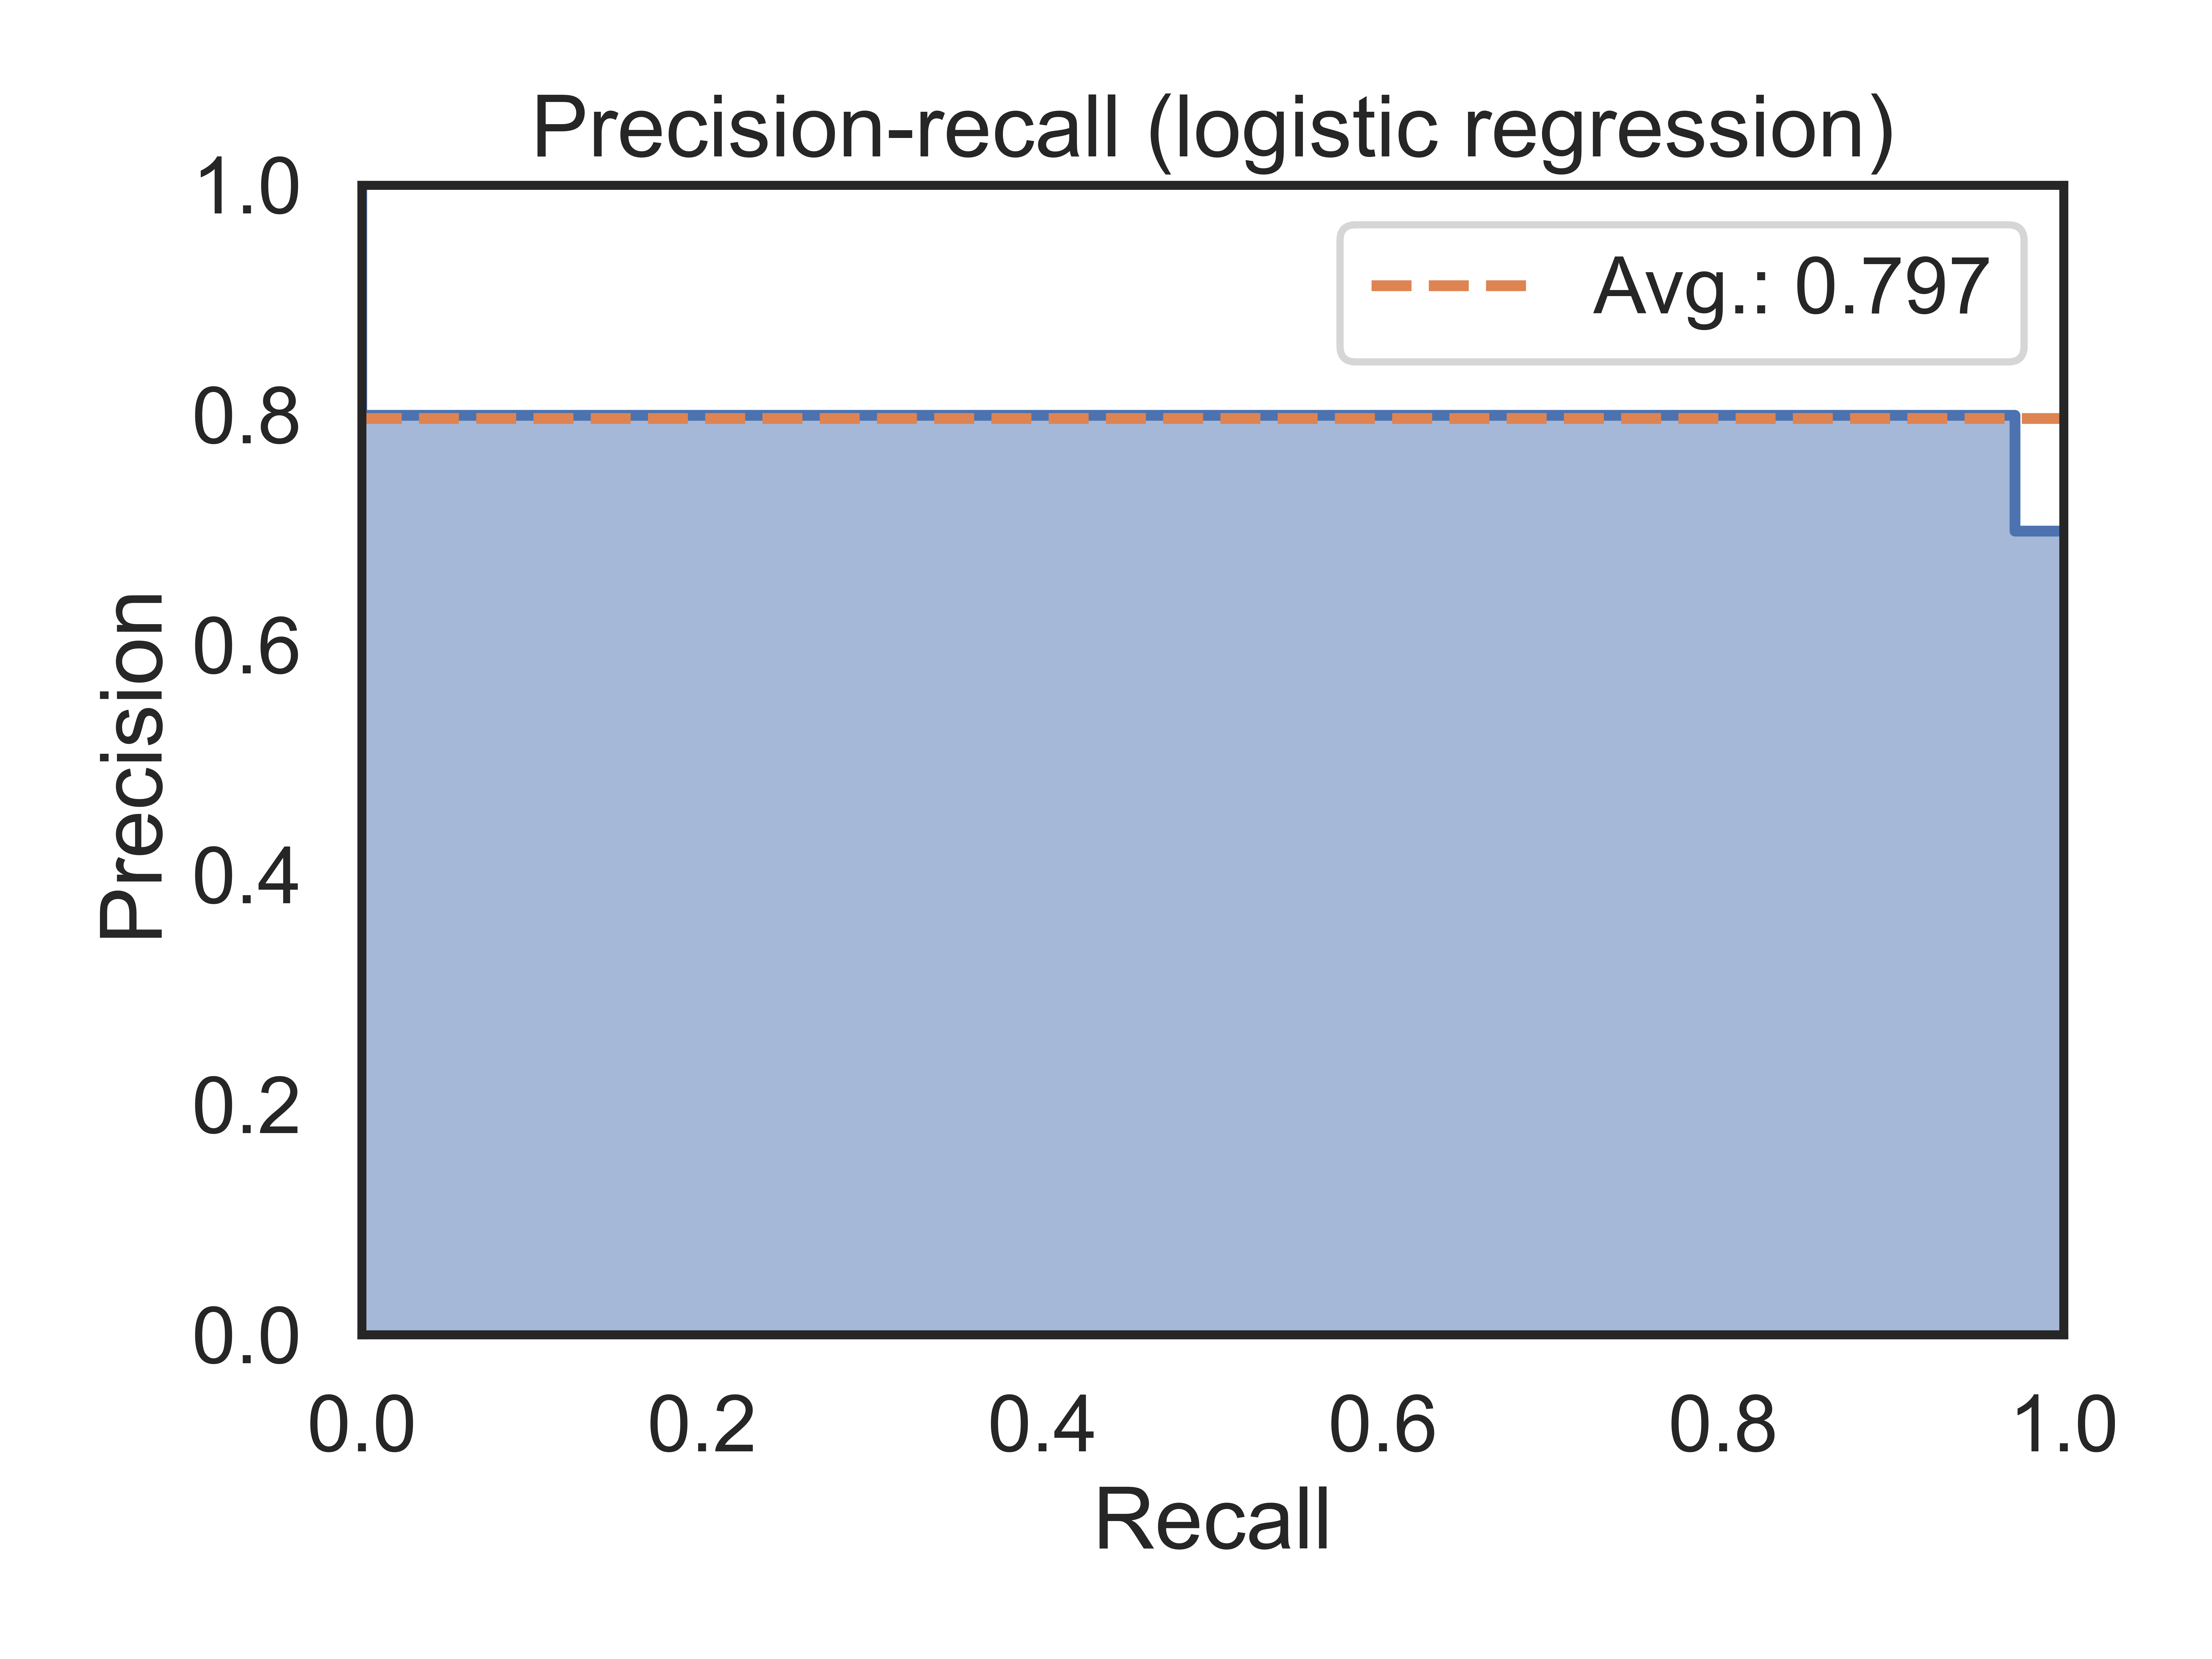
\includegraphics[width=0.95\textwidth]{./gfx/rq3/logistic_prc.png}
	\end{center}
	\caption{Precision-recall curve for logistic regression model}
	\label{fig:prc-logreg}
\end{figure}

The receiver operating characteristic curve for this model was also plotted.
It illustrates the rate of true positive predictions made by the model (Equation~\ref{eq:tpr}):

\begin{equation}
	\text{TPR} = \frac{T_p}{T_p + F_n}
	\label{eq:tpr}
\end{equation}

against the rate of false positive predictions made by the model (Equation~\ref{eq:fpr}):

\begin{equation}
	\text{FPR} = \frac{F_p}{F_p + T_n}
	\label{eq:fpr}
\end{equation}

where $F_p$ is the raw number of false positive predictions and
$T_n$ is the number of true negative predictions the model made.

\begin{figure}
	\centering
	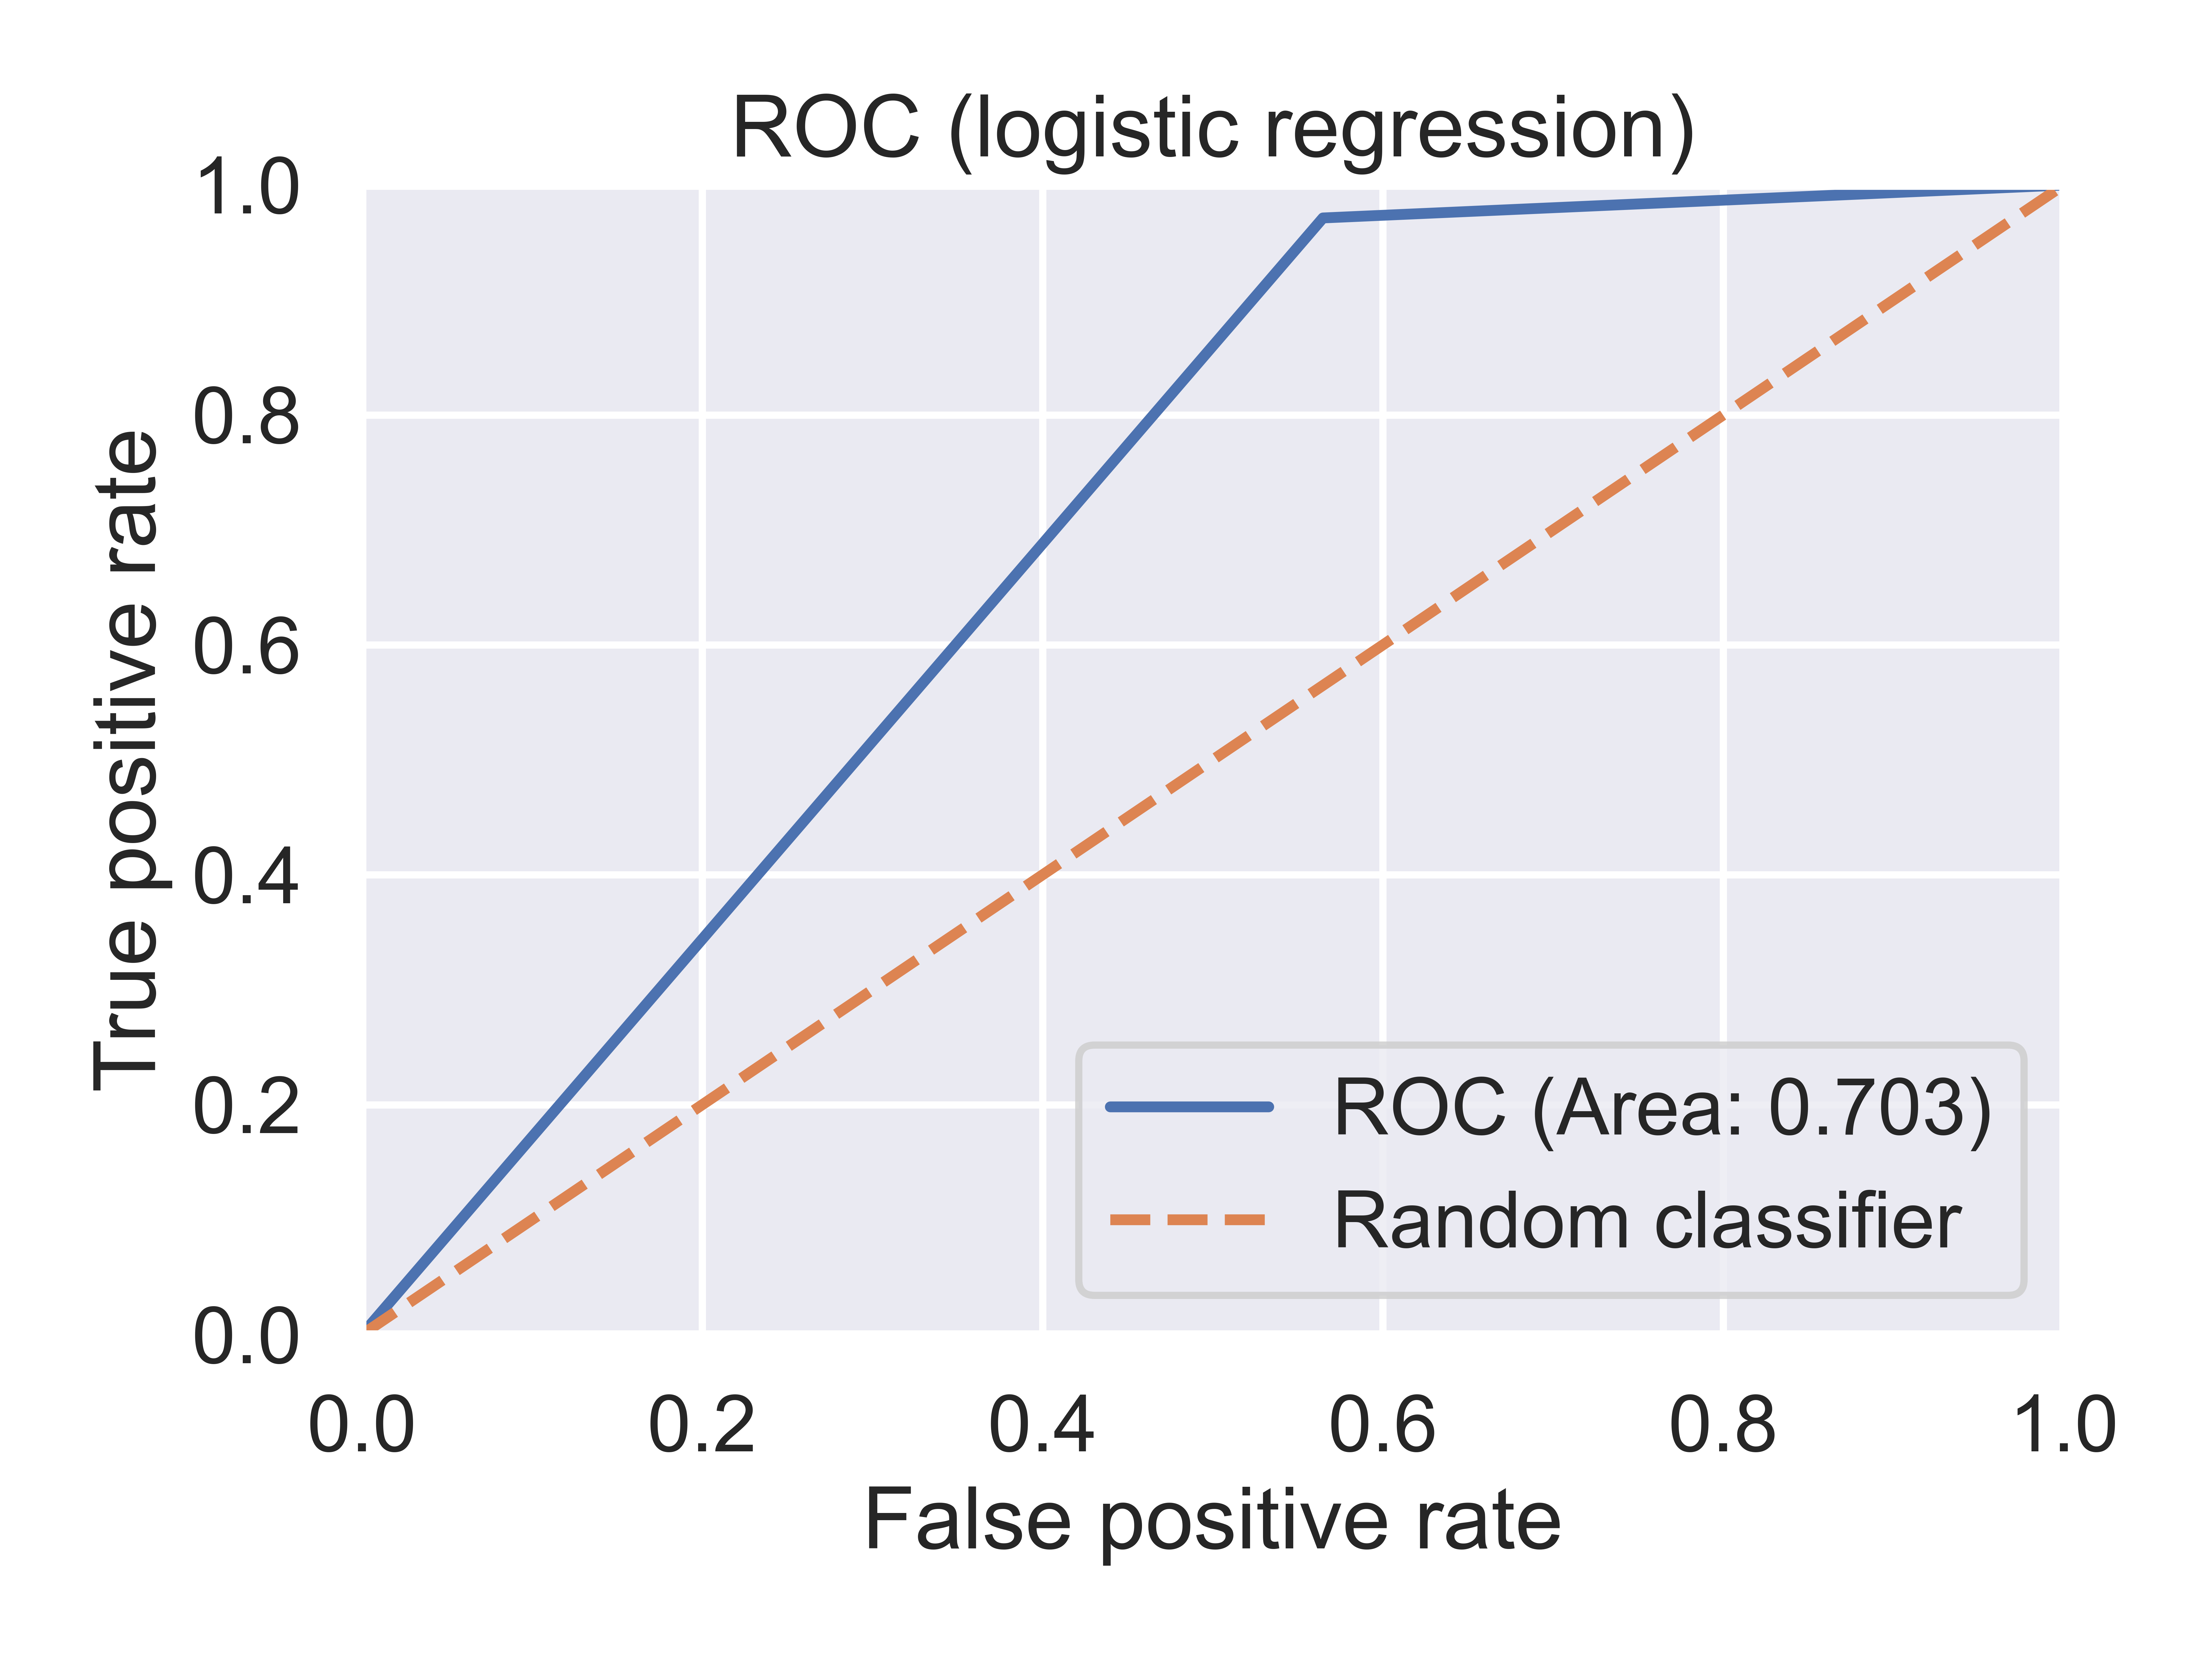
\includegraphics[width=0.95\textwidth]{./gfx/rq3/logistic_roc.png}
	\caption{Receiver operating characteristic curve for logistic regression model}
	\label{fig:roc-logreg}
\end{figure}

Comparing the performance of this model with a hypothetical
model that makes predictions randomly, the area under the receiver
operating characteristic (Figure~\ref{fig:roc-logreg}) curve is $0.70$,
thus the model model performs well at distinguishing positive and negative predictions.

\subsubsection{Random forest classifier}
A random forest classifier was also constructed to predict
the overall sentiment of a hotel review. It relies on feature
importance: how important tokens are in determining overall sentiment.

The model takes random samples from the dataset of hotel reviews
and then generates multiple decision trees. After which, it averages
out the results from each decision tree. As before, the precision-recall (Figure~\ref{fig:prc-rf})
and receiver operating characterstic curves (Figure~\ref{fig:roc-rf}) were plotted.

\begin{figure}
	\centering
	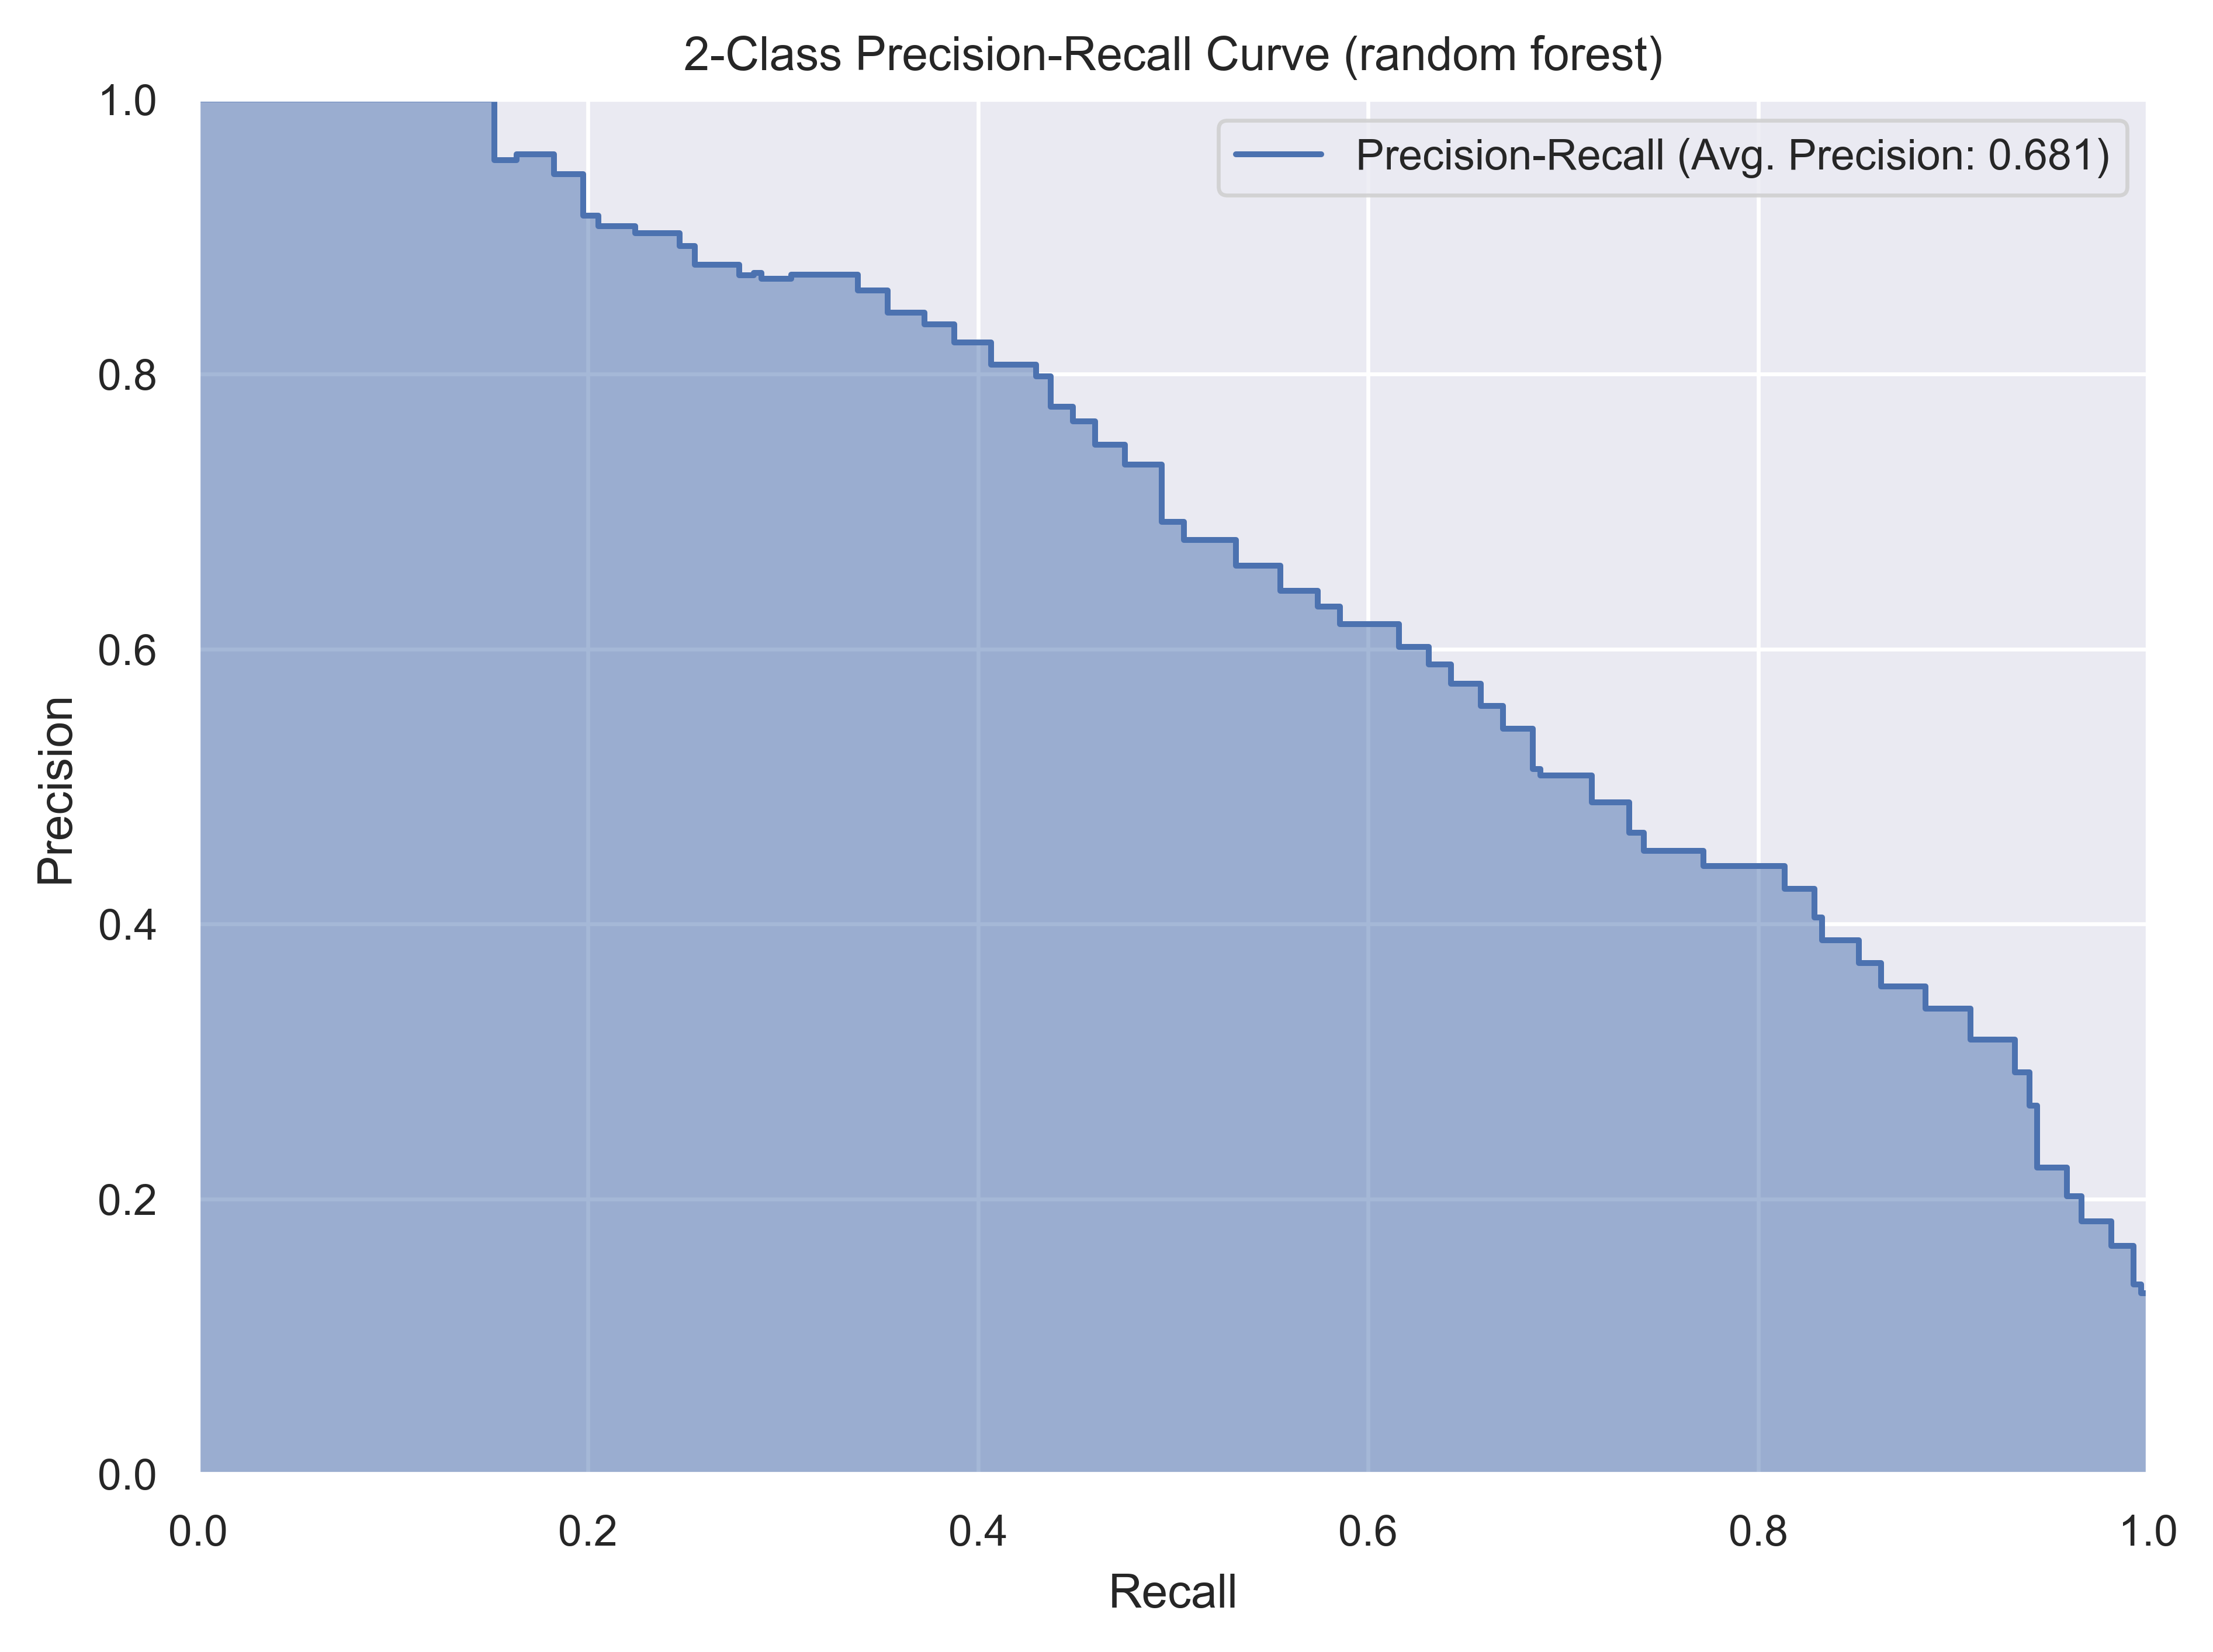
\includegraphics[width=0.95\textwidth]{./gfx/rq3/rndforst_prc.png}
	\caption{Precision-recall curve for random forest classifier}
	\label{fig:prc-rf}
\end{figure}

Figure~\ref{fig:prc-rf} reflects an average precision of $0.68$,
faring less well compared to the logistic regression model.

\begin{figure}
	\centering
	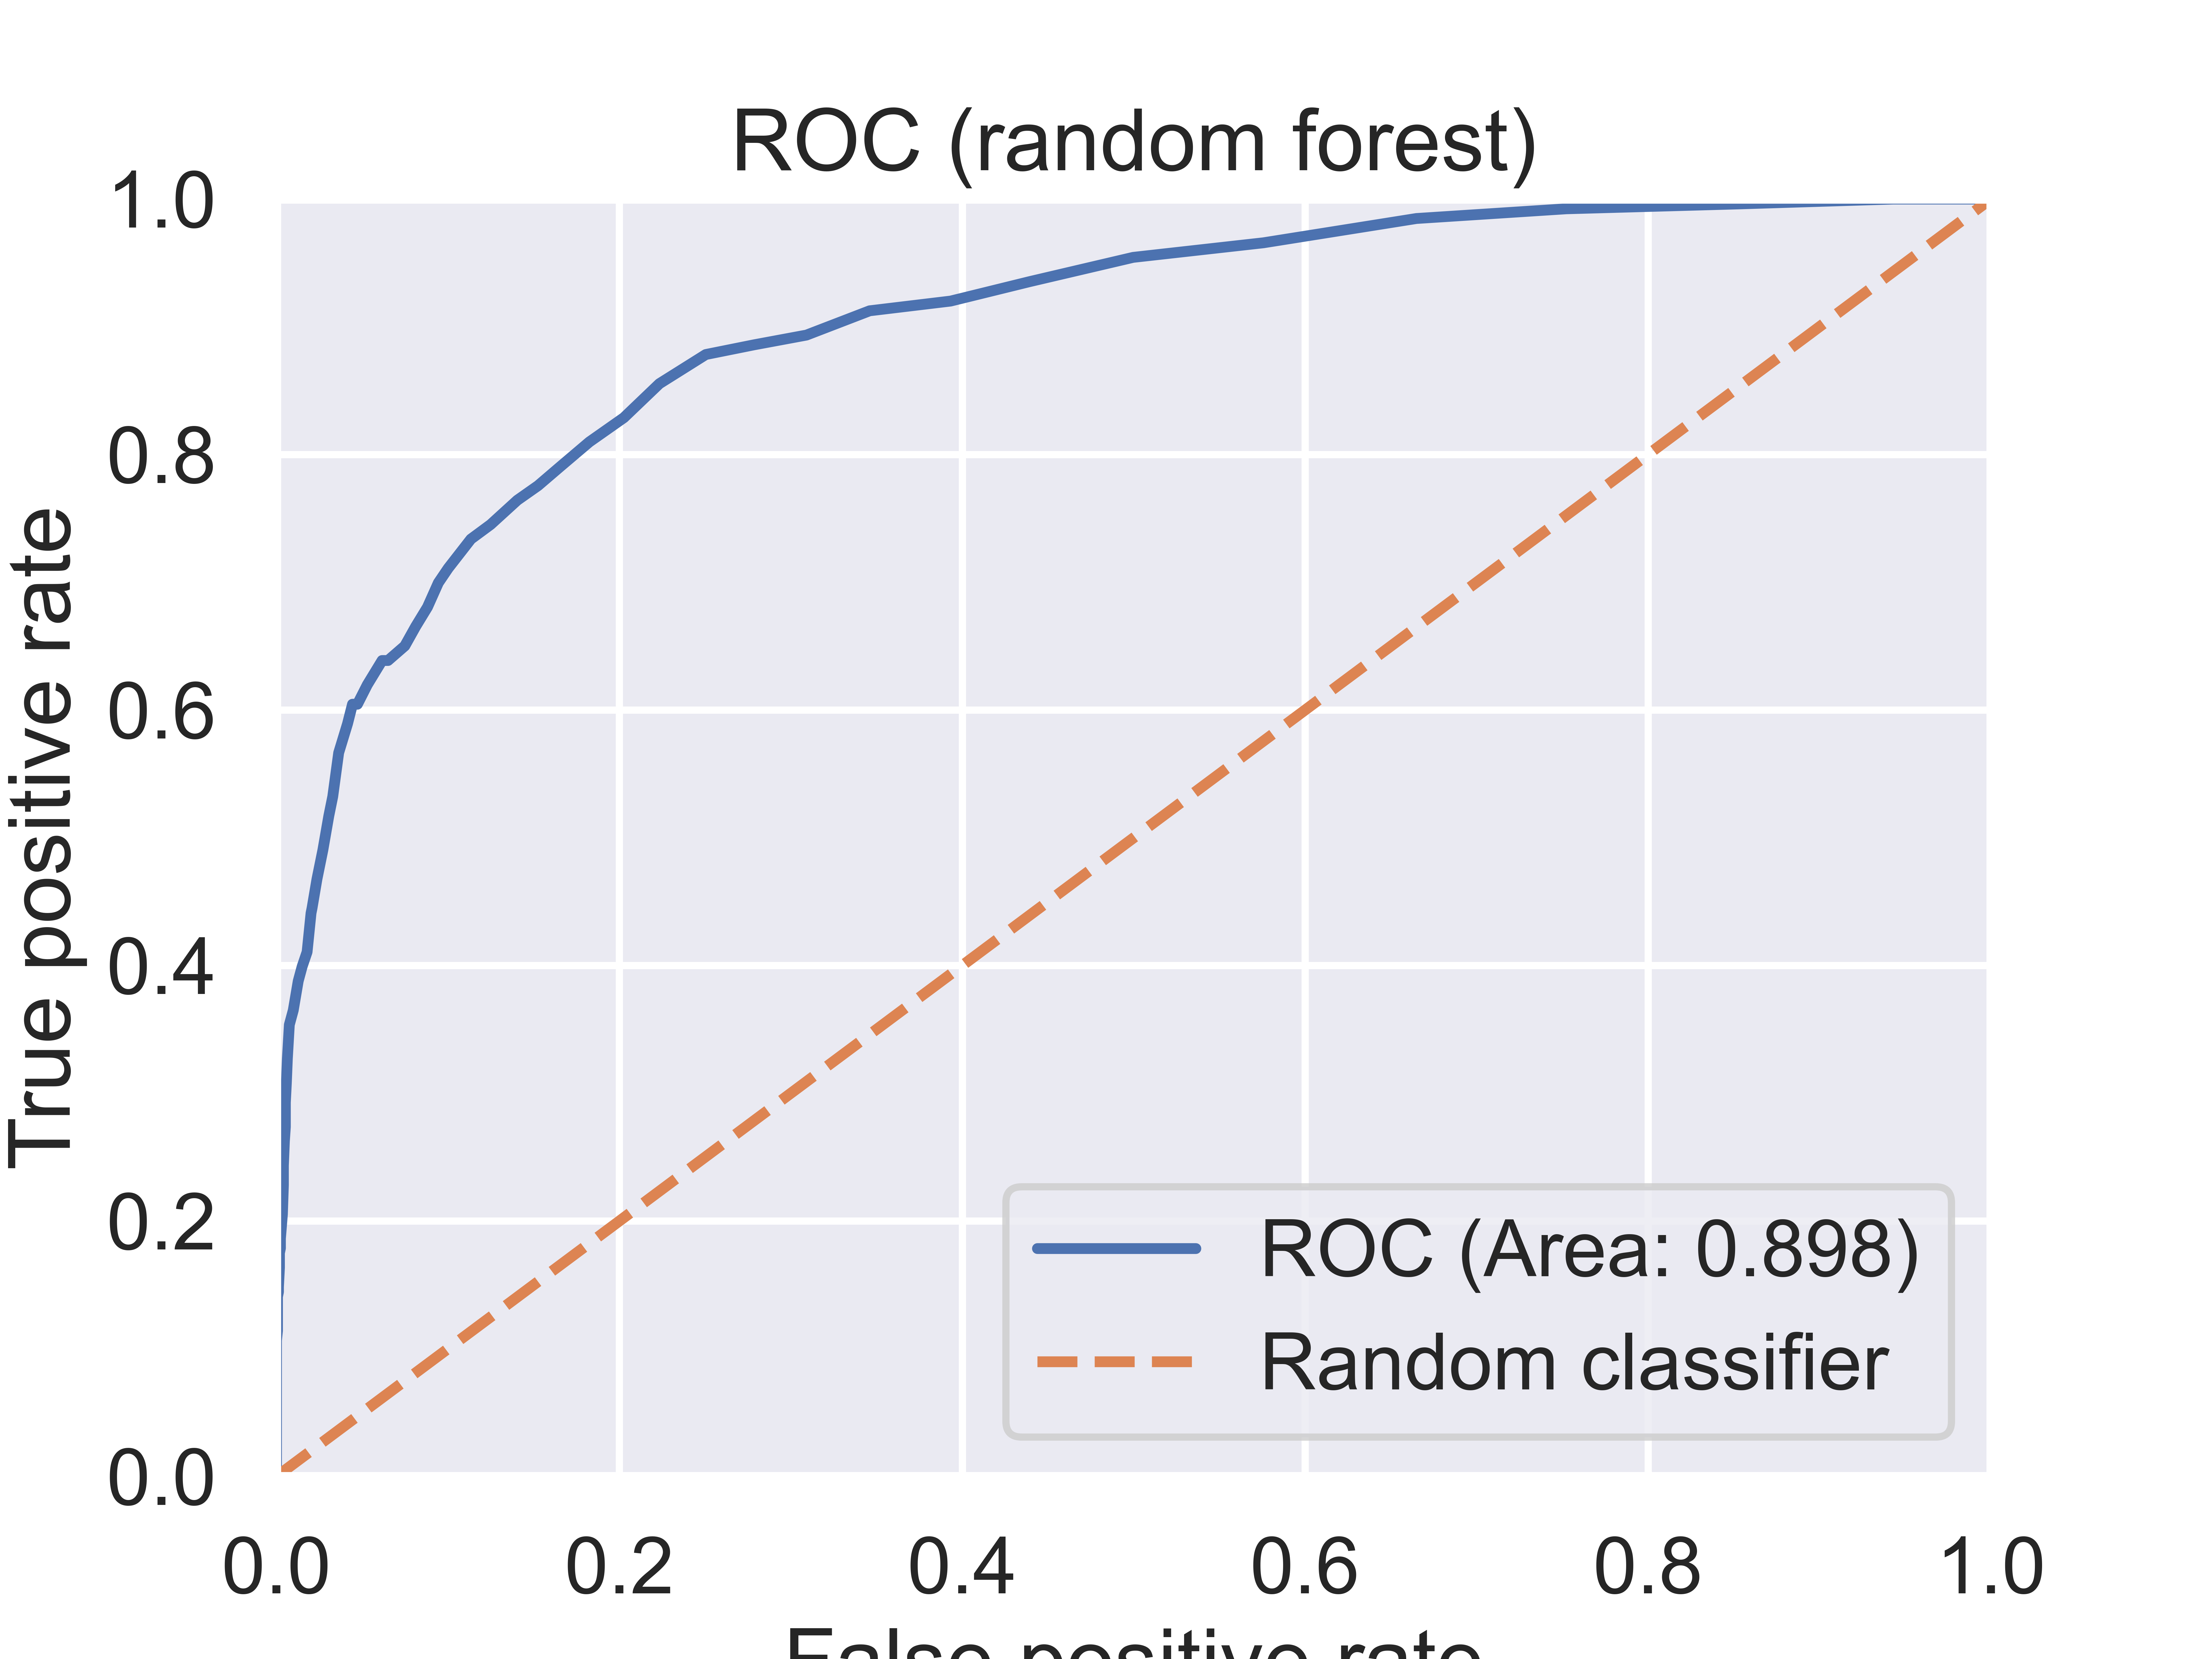
\includegraphics[width=0.95\textwidth]{./gfx/rq3/rndforst_roc.png}
	\caption{Receiver operating characteristic curve for random forest classifier}
	\label{fig:roc-rf}
\end{figure}

In contrast, Figure~\ref{fig:roc-rf} shows that the area under
the receiver operating characteristic curve is $0.90$, which means
that the random forest classifier performs better at distinguishing
true and false positive predictions than the logistic regression model.

\section{Discussion}

\subsection{Summary}

Sentiment analysis was performed on a dataset of international hotel reviews
in English. Hotel reviews were tokenised---split into individual words which
carry tangible meaning---and their sentiments were determined using a sentiment
lexicon. Although the majority of the lexicon contained neutral tokens,
such as \textit{hotel}, \textit{visit} and \textit{food}, the number of tokens
that carry positive sentiment far exceeds that with negative sentiment.

On a larger scale, the sentiments of individual hotel reviews were quantified
using SentiStrength, with positive reviews greatly outnumbering negative ones
by a considerable margin.

A logistic regression model and a random forest classifier were trained to
predict the sentiments of hotel reviews. Upon making predictions, the models
were found to have moderately high average precisions and high rates of
success in distinguishing false and true positive predictions. The logistic
regression model performed better than the random forest classifier in precision,
but the random forest classifier was more capable of distinguishing false and true
positive predictions.

\subsection{Limitations}
Homographs---words that have the same spelling but different meanings---could
not be distinguished during tokenisation (Section~\ref{sec:tokens}), resulting in
slightly unreliable sentiment scores. For instance, the word \textit{lobby} was shown to
carry a negative sentiment (Figure~\ref{fig:wordclouds}). However, the word \textit{lobby}
was only used to refer to a hotel lobby upon closer inspection.

Furthermore, the data collected was limited only to English international hotel reviews.
A more complete analysis of hotel reviews would include tourists of different language
backgrounds; hence, sentiment analysis would need to be conducted in more than one language.

While a random forest classifier generally gives more diverse results via random
selection of token frequencies, it fails to discover trends that would enable it to extrapolate
values that fall outside the training data. Instead, it relies on the average of all the results
of its decision trees instead, predicting a value always within the maximum and minimum sentiment scores.
A review that carries an overly positive or negative sentiment would produce unreliable results.

A logistic regression model, on the other hand, assumes that the tf--idf values of tokens
and the overall sentiment of a review are linearly related (because of the linear component $\beta_0 + \beta_1x_i$
in Equation~\ref{eq:sigmoid}), which may hinder the accuracy of the predictions it makes.

\subsection{Future Work}

Much can be done to extend this project, because of the relatively small scale on which this project
was conducted. As above, sentiment analysis could be conducted in more than one language (besides English)
to gain a broader understanding of tourists' preferences in hotels from different languages and cultural
backgrounds.

Furthermore, more prediction models could be constructed. This would create a larger
variation in the predictions made, enabling the precision of the models used in this project to be
compared with those of other models to evaluate the model with the highest accuracy. Constructing a
wider range of prediction models also allows for the possibility of more advanced techniques,
including Naïve Bayes prediction models or recurrent neural networks, both of which are
widely used in analysing sentiment from textual data. In particular, recurrent neural
networks perform better at analysing tokens in context, avoiding the issue
of unreliable sentiment scores described above.

% ** bibliography **
\printbibliography[heading=bibintoc]
\end{document}
